\documentclass[a4paper, 11pt]{article} % 11pt for better readability with standard fonts

% Packages
\usepackage{booktabs}
\usepackage{graphicx}
\usepackage{amsmath}
\usepackage{authblk}
\usepackage{appendix}
\usepackage{listings}
\usepackage{subcaption}
\usepackage{siunitx}
\usepackage{amsmath}
\usepackage{amssymb}
\usepackage[T1]{fontenc} % Ensures proper font encoding and crisp text
\usepackage[a4paper, margin=1in]{geometry}
\usepackage[dvipsnames]{xcolor}
\usepackage{tabularx}

% Hyperlink configuration (Keeps preferred hidelinks and cleveref setup)
\usepackage[hidelinks]{hyperref}
\usepackage[nameinlink, capitalise]{cleveref}

% Define 'Y' to be a left-aligned 'X' column to prevent underfull box warnings
\newcolumntype{Y}{>{\raggedright\arraybackslash}X}

% Code listing configuration
\lstset{ 
    language=Python,               
    keepspaces=true,
    columns=fullflexible,
    backgroundcolor=\color{white},  
    basicstyle=\ttfamily, 
    showstringspaces=false,
    keywordstyle=\color{blue},      
    commentstyle=\color{ForestGreen},     
    stringstyle=\color{red},        
    breaklines=true,                
    captionpos=b,                   
    numbers=left,                   
    numberstyle=\tiny\color{gray}   
}

% Bibliography setup
\usepackage[backend=biber,style=apa]{biblatex}
\addbibresource{references.bib}

\begin{document}

% ==========================================
%               TITLE PAGE
% ==========================================
\begin{titlepage}
    \centering
    \vspace*{1cm}
    
    {\Large\bfseries Imperial College London \par}
    {\large Department of Earth Science and Engineering \par} % Update to your specific department
    {\large MSc Environmental Data Science and Machine Learning \par} % Update course name
    
    \vspace{2.5cm}
    
    {\LARGE\bfseries Comparison of Direct and Cascaded High-Resolution Spatial Downscaling of Wildfire Data \par}
    
    \vspace{2.5cm}
    
    {\large\bfseries Author:} \\
    {\large Tsuyu Huang} \\
    {\small \href{mailto:tsuyu.huang25@imperial.ac.uk}{tsuyu.huang25@imperial.ac.uk} \par} % Replace with your email
    
    \vspace{1cm}
    
    {\large\bfseries Supervisors:} \\
    {\large Jorge Veiras (\href{mailto:jorge@artiocarbon.com}{jorge@artiocarbon.com})} \\
    {\large Prof. Anna Korre (\href{mailto:a.korre@imperial.ac.uk}{a.korre@imperial.ac.uk}) \par}

     \vspace{1.5cm}
    
    % Repository links formatted as clickable text matching your hyperref preferences
    {\large\bfseries Code Repository:} \\
    {\small \url{https://github.com/ese-ada-lovelace-2025/irp-th25} \par} 

    \vspace{1.5cm}
    
    {\large\bfseries Company:} \\
    {\large Artio} \\
    {\small \href{https://www.artiocarbon.com/}{www.artiocarbon.com} \par}
    
    \vfill
    
    {\large \today \par}
\end{titlepage}

\nopagebreak

% ==========================================
%          ABSTRACT & CONTENTS
% ==========================================
\begin{abstract}
With climate change, high-resolution wildfire data is increasingly vital for risk assessment. This project investigates deep learning for downscaling GOES imagery ($2\,\text{km}$) to Landsat-resolution fire masks ($30\,\text{m}$), incorporating topographic and land cover covariates to address extreme class imbalance and $66\times$ resolution gap. We evaluate whether cascaded pipeline (GOES $\to$ VIIRS $375\,\text{m}$ $\to$ Landsat) outperforms direct pipeline (GOES $\to$ Landsat), comparing a Hybrid Attention U-Net (HAUNet) against an Autoencoder baseline. All configurations capture genuine fire signals, achieving up to $30\times$ higher AUPRC than prevalence-rate reference. Direct downscaling yields higher overall confidence ranking across both architectures (e.g. HAUNet AUPRC $0.0188$ direct vs. $0.0142$ cascaded), whereas cascading improves thresholded spatial overlap metrics, most prominently for HAUNet (IoU $0.0072$ vs. $0.0044$ direct): indicating no pipeline is uniformly superior. HAUNet outperforms Autoencoder across both pipelines, and feature ablations confirm elevation covariates contribute to performance. Results indicate the models are better suited for coarse regional risk flagging than precise fire-area prediction, with direct relevance to practical risk applications where under-prediction is costlier than over-prediction.
\end{abstract}

% ==========================================
%     DECLARATION OF AI TOOLS
% ==========================================
\section*{Declaration of Generative AI Tools}
\addcontentsline{toc}{section}{Declaration of Generative AI Tools}

The content and critical analysis presented in this report were written by the student without generative AI.

Generative AI models (\href{https://gemini.google.com/app}{Google Gemini 3.6}, \href{https://claude.ai/new}{Anthropic Claude Sonnet 5}) were used as developer tools during software implementation. This usage was restricted to:

\begin{itemize}
    \item \textbf{Code Generation \& Modularisation:} Drafting code, modularising scripts, and creating visualisation tools.
    \item \textbf{Debugging \& Cloud Integration:} Troubleshooting execution errors, optimisation, and assisting with using Google Cloud Services.
    \item \textbf{Implementation Ideation:} Exploring architectural configurations and workflow design possibilities.
\end{itemize}

Generated codes were manually reviewed, modified, and integrated by the author. References detailing AI usage is in the project repository at \texttt{references.md}.

\clearpage

\tableofcontents
\clearpage

% ==========================================
%             MAIN CONTENT
% ==========================================
\section{Introduction}
Rising Net-Zero investment has driven funding for carbon-reduction projects such as reforestation (\cite{InvestmentTrendsOutcomes}), which are increasingly at risk from wildfires that release stored carbon back into the atmosphere as fire frequency and severity escalate with climate change (\cite{jonesClimateChangeIncreases}). This causes economic losses for the insurance industry. e.g. The January 2025 Los Angeles County wildfires set an all-time record, causing \$40 billion in insured losses (\cite{staffHowWildfiresStorms2026}). In carbon accounting, underestimating fire area leaves projects underinsured, whereas overestimation is conservative (\cite{grassiApplyingConservativenessPrinciple2008}). This project, conducted with Artio, aims to provide higher-resolution fire data to give better confidence and risk assessment for insurance industry.

Accurate risk assessment requires wildfire data that is both high-spatial and high-temporal resolution. Geostationary (GEO) satellites provide high-temporal frequency but coarse spatial resolution, while Low Earth Orbit (LEO) satellites offer high spatial detail at low temporal frequency. Existing Deep Learning (DL) downscaling methods bridge this trade-off, but the resolution gap between GEO ($2\,\text{km}$) and LEO ($30\,\text{m}$) is extreme: a single $2\,\text{km}$ GOES pixel covers roughly $4,444$ Landsat $30\,\text{m}$ pixels. This is an ill-posed, one-to-many super-resolution task prone to physically implausible outputs.

To mitigate this limitation, this project integrates additional physical information, such as high-resolution topography and landcover to guide downscaling. The project aims to investigate whether cascaded downscaling ($2\,\text{km}$ to $375\,\text{m}$ to $30\,\text{m}$) produces better results compared to direct downscaling ($2\,\text{km}$ to $30\,\text{m}$). By breaking up the downscaling process, the model trains on a smaller resolution gap, aiming to mitigate error caused by large resolution gaps. This project will compare cascaded and direct pipeline performance of downscaling architectures (hybrid attention U-Net and Autoencoder).

\section{Current State of Remote Sensing Downscaling}
Traditional downscaling methods often fail to capture the complex non-linear patterns in remote sensing data. DL methods have shown to outperform these approaches (\cite{sdrakaDeepLearningDownscaling2022}). CNN and U-Net architectures have been widely used for their spatial feature extraction, GAN-based methods where sharpness is prioritised over pixel accuracy, and transformer-based and diffusion-based approaches more recently demonstrating strong long-range and generative capability respectively (\cite{wangVGGTVisualGeometry2025, wangSinSRDiffusionBasedImage2023}).

However, many architectures are optimised for texture-rich, natural images, and not designed for extreme resolution-gaps ($66.7\times$ in this project). They may perform poorly on active wildfire data, where the target signal is extremely sparse and localised. In risk assessment, fire mask is preferred for direct analysis. This creates two challenges: severe class imbalance that biases standard reconstruction loss functions (\cite{qiAdvancingImageSuperresolution2026}); and an ill-posed one-to-many mapping (\cite{wangDeepLearningImage2020}). Architectures are needed that can preserve fire signal against a dominant background and recover coherent fire-front structure.

Closest precedents to this task are \cite{mccarthyDeepLearningApproach2021} and \cite{badhanDeepLearningApproach2024}: trained a U-Net and autoencoder respectively to downscale GOES observations to VIIRS-equivalent $375\,\text{m}$ fire mask. Both stop at $375\,\text{m}$ resolution, leaving the challenge of downscaling to $30\,\text{m}$ resolution unaddressed.

While wildfires are influenced by factors like terrain and landcover (\cite{sullivanInfernoFundamentalProcesses2017}), generic super-resolution models omit this information. Providing high-resolution covariates provides context and constraints for the model, which may help mitigate the ill-posed nature of the downscaling problem.

Models downscaling across large resolution-gaps using coarse thermal imagery alone are constrained by satellite physical detection limits. Validation of GOES-16 against $30\,\text{m}$ Landsat-8 data demonstrates that the active fire detection probability reaches $95\%$ only when coarse $2\,\text{km}$ area contains at least $114$ active Landsat sub-pixels (\cite{liPreliminaryEvaluationGOES162020}). Detection probability drops below this threshold, coarse channels frequently carrying zero detectable signal for smaller fires. The equivalent $95\%$ detection for VIIRS $375\,\text{m}$ requires only 11 active sub-pixels, reducing signal threshold. This motivates staged downscaling: training on smaller resolution-gap, and intermediate VIIRS stage operating at lower detection threshold, meaning the input carries genuine signal where the direct downscaling may not.

Existing literature is dominated by direct downscaling across the full resolution gap. Comparisons of multi-stage pipelines also remain scarce. \cite{liStepwiseDownscalingERA5Land2025} demonstrated that stepwise downscaling of ERA5-Land air temperature ($10.5\,\text{km} \rightarrow 30\,\text{m}$) outperformed direct downscaling. However, they evaluated meteorological variables using tree-based ensembles. To date, no prior work researches cascaded DL downscaling, particularly for wildfire applications. Nor has existing work explored the trade-off between reduced per-stage resolution gap and the use of independent intermediate satellite ground-truths across stages.

Main project objectives are:
\begin{enumerate}
    \item Develop and evaluate a downscaling framework tailored for active wildfires at $30\,\text{m}$ resolution, beyond $375\,\text{m}$, that exceeds the no-skill prevalence-rate reference-point under the extreme class imbalance and resolution gap in this task.
    \item Quantify whether attention-based architecture (HAUNet) achieves higher AUPRC and overlap-based metrics than a simpler Autoencoder baseline under matched training conditions, isolating the contribution of HAUNet's attention mechanisms.
    \item Determine whether cascaded pipeline with intermediate VIIRS stage achieves higher metrics than direct downscaling, quantifying trade-offs between reduced per-stage resolution gap that remains unexplored in literature.
\end{enumerate}

\section{Data and Materials}\label{sec:data}
Table \ref{tab:data_sources} shows the data sources for this project. The specifications for the VIIRS, GOES, and Landsat data are outlined in Table \ref{tab:pipeline_configs}.

The GOES-16/17 data were obtained via public Google Cloud Platform (GCP) buckets (\cite{noaa_goes16_gcp, noaa_goes17_gcp}). DEM, and ESA WorldCover are obtained via Google Earth Engine (GEE) Python API (\cite{gorelickGoogleEarthEngine2017}) and exported directly to Google Cloud Storage (GCS). The Landsat-8 fire masks are derived by \cite{dealmeidapereiraActiveFireDetection2021} and obtained from the author's public dataset (via Google Drive) and re-uploaded to GCS. VIIRS fire detections are obtained from NASA FIRMS archive. Manifests, split assignments and model checkpoints are also stored in GCS. 

There are $12,504$ and $1,202$ total VIIRS and Landsat patches respectively. The asymmetry in sample counts is due to different sources: Landsat from pre-existing external dataset, VIIRS generated directly from a larger available archive. This gives Stage 1 (GOES $\to$ VIIRS) of the cascaded pipeline a larger, more reliable training set, since Stage 1 errors propagate directly into Stage 2's input. But the final 30m downscaling is trained on the same Landsat dataset.

The data was processed so all regions of interest (ROIs) are dynamically reprojected to their localised UTM zone based on centroid coordinates. Detections from the NASA VIIRS S-NPP archive were filtered for "nominal" and "high" confidence points. Detections are clustered into $7680 \times 7680\,\text{m}$ grid cells within a 15-minute window of peak activity. VIIRS grid cell pixels record the peak Fire Radiative Power (FRP). Due to extreme class imbalance of the target fire datasets (mean fraction of positive target pixels are $0.85\%$ for VIIRS, $0.06\%$ for Landsat), stratified sampling was applied across temporal extent and fire pixel count bins during data splitting. The closest temporal GOES-16/17 scan within a $\pm 60$-minute guard window was queried (assuming fire spread is stable within that window at $2\,\text{km}$ resolution).

GOES-16/17 channels 7 ($3.9\,\mu\text{m}$, shortwave IR) and 14 ($11.2\,\mu\text{m}$, longwave IR) are used as they correspond to the spectral bands for fire-detection for their sensitivity to fire radiance. Similar spectral logic applied in VIIRS's active-fire algorithm, which similarly relies on a shortwave (I4, $3.74\,\mu\text{m}$) and longwave (I5, $11.45\,\mu\text{m}$) channel pair. (\cite{schmidtGOESRAdvancedBaseline})

In addition to $3.9\ \mu\text{m}$ (Ch. 7) and $11.2\ \mu\text{m}$ (Ch. 14) GOES brightness temperatures, a Thermal Fire Index (TFI) is computed as additional input channel:

\begin{equation}
    TFI = Ch.7 - Ch.14
    \label{eq:tfi}
\end{equation}

Explicitly providing TFI reduces the burden on early network layers to discover a known, physically meaningful relationship, aiming to save model capacity and improving convergence.

\begin{table}[htbp]
\centering
\small
\caption{Data Sources and Specifications}
\label{tab:data_sources}
\begin{tabularx}{\textwidth}{lccY}
\hline
\textbf{Data Source} & \textbf{Res.} & \textbf{Bands Used} & \textbf{Role / Context} \\ \hline
Landsat-8 Fire Masks & 30 m & Active Fire Mask \cite{dealmeidapereiraActiveFireDetection2021} & Target / ground truth; binary mask ($256\times256$ px) \\
VIIRS S-NPP & 375 m & I4 (3.74~$\mu$m, Active Fire) & Intermediate target / cascaded-pipeline input (FRP, NASA FIRMS) \\
GOES-16/17 (ABI) & 2000 m & Ch.\,7 (3.9~$\mu\text{m}$), Ch.\,14 (11.2~$\mu\text{m}$) & Coarse fire input; brightness temperature, high temporal frequency \\
Copernicus DEM & 30 m & DEM & Static covariate; terrain effects on fire spread \\
ESA WorldCover & 10 m & Landcover (10 classes) & Static covariate; land cover map \\ \hline
\end{tabularx}
\end{table}

\begin{table}[htbp]
\centering
\small
\caption{Data Pipeline Configuration Specifications}
\label{tab:pipeline_configs}
\begin{tabularx}{\textwidth}{lcY}
\hline
\textbf{Parameter} & \textbf{Value} & \textbf{Description} \\ \hline
VIIRS Geographic Bounds & $[-170.0, -30.0]$ & Longitude limits for the Americas \\
VIIRS Date Range & 2020-01-01 -- 2020-12-31 & Temporal query window for VIIRS detections \\
Landsat Geographic Bounds & N.\ \& S.\ America & Locations of interest for GOES detections \\
Landsat Date Range & Aug--Sep 2020 & Temporal window for Landsat detections \cite{dealmeidapereiraActiveFireDetection2021} \\
Min.\ Landsat Active Pixels & $10$ & Minimum active fire pixels to retain a patch \\
GOES Temporal Guard & 60 min & Max.\ gap between target time and GOES scan \\
GOES Native Scale & 2000 m & Native GOES ABI grid spacing \\
Landsat Grid Scale & 30 m & Resolution, Landsat branch \\
VIIRS Grid Scale & 375 m & Resolution, VIIRS active fire detections \\
Landsat Dimensions & $256 \times 256$ px & Target patch size \\
VIIRS Dimensions & $20 \times 20$ px & Target size ($7680/375$) \\
GOES Dimensions & $4 \times 4$ px & Target size ($7680/2000$) \\ \hline
\end{tabularx}
\end{table}

\section{Methods}

\subsection{HAUNet (Hybrid Attention U-Net)}
Among CNN-based approaches, HAUNet (\cite{wangHybridAttentionBasedUShaped2023}) uses hybrid attention to capture both local fine detail and broader contextual structure across multiple scales.

\subsubsection{Hybrid Attention Mechanisms}
\begin{itemize}
    \item \textbf{Channel Attention Module (CEM):} Computes channel dependencies with $O(C^2)$ complexity. Given feature map $\mathbf{X} \in \mathbb{R}^{C \times H \times W}$, queries $\mathbf{Q}$, keys $\mathbf{K}$, and values $\mathbf{V}$ are generated via $1 \times 1$ convolutions followed by $3 \times 3$ depthwise convolutions. The channel attention map $\mathbf{A}_c$ is derived as:
    \begin{equation}
        \mathbf{A}_c = \text{Softmax}\left(\text{ReLU}\left(\frac{\mathbf{Q} \mathbf{K}^T}{\alpha}\right)\right) \mathbf{V}
    \end{equation}
    where $\alpha$ is a learnable scaling parameter.
    
    \item \textbf{Spatial-Channel Attention (S\_CEM):} Parallel spatial attention branch operating along transposed dimensions $\mathbf{Q}_s, \mathbf{K}_s, \mathbf{V}_s \in \mathbb{R}^{B \times N_{head} \times HW \times C}$. The full spatial attention step scales quadratically with spatial resolution as $O((HW)^2)$.
\end{itemize}

\subsubsection{Full-Resolution Covariate Pyramid Branch}
The original \cite{wangHybridAttentionBasedUShaped2023} HAUNet applies full spatial attention in S\_CEM with $O((HW)^2)$ memory footprint that causes out-of-memory errors on full-resolution inputs. Hence inputs ($256 \times 256$) are downsampled by factor $D=4$ (i.e. $256/4 = 64$) before passing to the model.

The parallel Covariate Pyramid Encoder was introduced as modification to the original HAUNet because downsampling input covariates discards the high-resolution detail at $30\,\text{m}$ scale. It processes covariates at full-resolution in a separate branch, then progressively fusing into the main decoder path. This branch uses Windowed Spatial-Channel Attention Blocks (Windowed-S\_CEM) (\cite{liuSwinTransformerHierarchical2021}) for computational efficiency.

For a feature map partitioned into non-overlapping local windows of size $P \times P$ ($P=8$), Windowed-S\_CEM computes spatial attention independently within each window. The window is shifted sequentially with size $P/2$. This keeps spatial attention complexity to $O(P^4)$ per window, independent of overall spatial input dimensions.

\subsubsection{Multi-Scale Refinement and Feature Fusion}
The main encoder-decoder path produces low-resolution feature representations ($64 \times 64$). The final refinement stage produces the final high-resolution output. At each refinement stage, low-resolution features are upsampled (bilinear interpolation, $3\times3$ convolution), concatenated with matching-scale Covariate Pyramid Encoder features, and fused via a $3\times3$ convolution back to the working channel dimension.

The final layer of HAUNet refinement network outputs prediction at the resolution of the full covariate grid ($256 \times 256$). Operating the decoder at full resolution preserves fine-grained spatial feature representations across skip connections and covariate channels. This is same for Stage 1 (GOES $\to$ VIIRS) model output for cascaded pipeline. Rather than constraining the output's resolution to match the coarse VIIRS target grid ($20 \times 20$), HAUNet outputs high-resolution spatial feature maps. During metric evaluatation of the Stage 1 model, the outputs are pooled to VIIRS resolution to match VIIRS target.

\subsubsection{Cross-scale Interaction Module (CIM)}
HAUNet replaces standard skip-connections with Channel Interaction Module (CIM) to resolve semantic mismatches across encoder stages. Encoder features ($F_1, F_2, F_3$) are upsampled to equal dimensions $T_1, T_2, T_3$ and concatenated into a multiscale token $T_\Sigma \in \mathbb{R}^{H \times W \times 3C}$. CIM computes channel cross-attention ($Q_i K^T$) using $T_i$ as Queries and $T_\Sigma$ as Keys/Values, letting each scale aggregate cross-level context before element-wise addition into decoder blocks.

\begin{figure}[htbp]
    \centering
    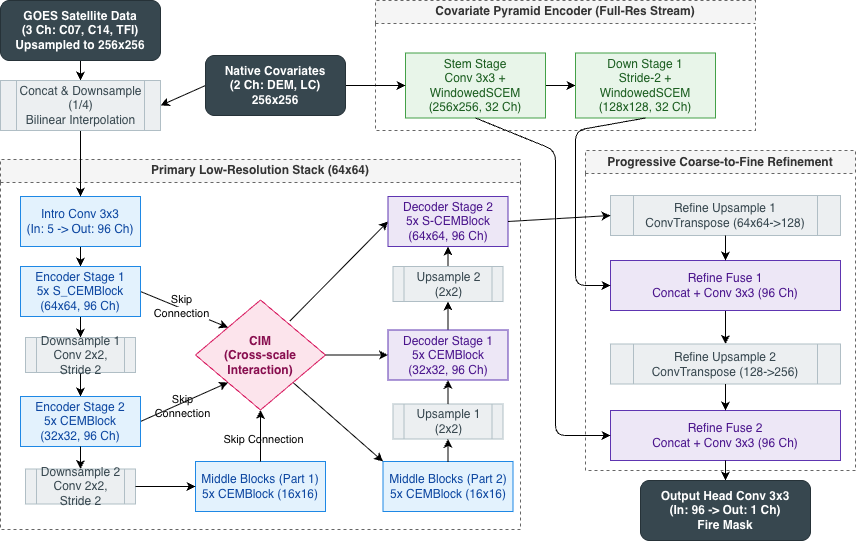
\includegraphics[width=\linewidth]{figures/haunet_diagram.png}
    \caption{Architecture overview of the wildfire-adapted HAUNet. The full-resolution stream processes native covariates, which are progressively fused via refinement blocks with the low-resolution stack after CIM.}
    \label{fig:haunet}
\end{figure}

\subsubsection{Architecture Selection Rationale}
HAUNet was selected as one of the architectures for the following reasons: 
\begin{enumerate}
    \item Dual attention: channel attention to capture global information across feature channels and spatial attention to capture spatial relationships. This is useful for wildfire data, where the fire signal is sparse and localised, but the physical context (e.g. terrain, landcover) is important for accurate downscaling.
    \item CIM: standard skip-connections concatenate features at matching spatial resolution, but this assume they are semantically comparable. CIM addresses this by explicitly bridging semantic and resolution gaps between encoder outputs at different scales prior to fusion. This helps to better learn representation at different scales, which is useful for super-resolution tasks like this (downscaling by $66.7\times$).
    \item Both the autoencoder baseline (\ref{sec:autoencoder}) and HAUNet share similar underlying encoder-decoder with skip-connections structure. This allows the comparison between the two models to isolate the contribution of HAUNet's attention mechanisms and skip-connection design.
\end{enumerate}

\subsection{Autoencoder Baseline}\label{sec:autoencoder}
The baseline architecture follows the autoencoder proposed by \cite{badhanDeepLearningApproach2024} to downscale from GOES to VIIRS resolution. It is adapted to this project to concatenate the covariates with fire data inputs, and outputs are fire mask segmentation rather than continuous BT values. The autoencoder follows a standard U-Net-style structure, shown in Figure \ref{fig:autoencoder}.

\begin{figure}[htbp]
    \centering
    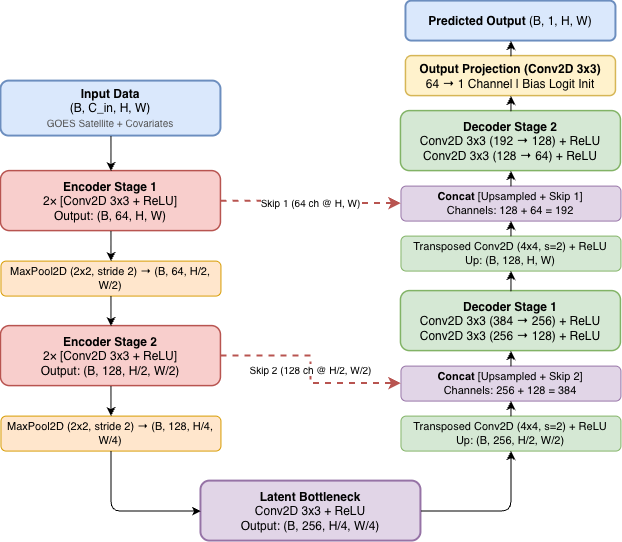
\includegraphics[width=\linewidth]{figures/autoencoder_diagram.png}
    \caption{Architecture overview of the autoencoder baseline based on \cite{badhanDeepLearningApproach2024}.}
    \label{fig:autoencoder}
\end{figure}

This baseline is trained under identical conditions to HAUNet (loss, optimiser, splits, covariates), isolating whether any performance gap is attributable to HAUNet's attention mechanisms rather than a simpler convolutional model.

\subsection{Loss Functions}
\subsubsection{Focal Dice Loss}
Active fire pixels represent a small fraction of each patch, resulting in extreme class imbalance. To address this, Focal Dice Loss was used (\cite{wangFocalDiceLoss2018}). While Focal loss forces the model to focus on hard-to-classify pixels, the Dice component maximises spatial region overlap. It combines Focal Loss (which down-weights background pixels via $(1-p_t)^\gamma$) with Dice Loss:

\begin{equation}\label{eq:focaldiceloss}
    \mathcal{L}_{\text{FD}} = w_f \cdot \mathcal{L}_{\text{focal}}(\alpha, \gamma) + w_d \cdot \mathcal{L}_{\text{dice}}
\end{equation}

where $w_f$ and $w_d$ are weights of the losses, $\alpha \in [0, 1]$ balances positive and negative pixel contributions, and $\gamma \ge 0$ controls the rate at which pixels are down-weighted. Full formulations are given in \ref{app:losses}.

The hyperparameters used are: $\alpha = 0.85, \gamma = 1.5, w_f = 1.0, w_d = 1.0$, which was assigned for final model training after tuning with subset of training samples ($1,000$). A higher $\alpha$ was assigned to penalise false negatives more heavily given the extreme class imbalance.

\subsection{Training Setup}
The dataset was split into training/validation/testing (80/10/10). Split uses stratified random sampling across four quantile bins based on the active pixel count for balanced representation. Weighted random sampling was applied during training to address class imbalance, where sample weights $w_i$ for each patch $i$ were assigned based on the count of positive fire pixels $n_i$:

\begin{equation}\label{eq:weighted_sampling}
    w_i = \max(n_i, 1)
\end{equation}

Note: This biases training toward larger fires, which is reasonable for Artio's use case since larger fires represent more insured exposure, though reported metrics should not be read as uniformly representative of small-fire performance. Evaluation metrics are unweighted per-patch means, so performance reflects average behaviour across all fire sizes.

Inputs are scaled prior to model ingestion. The GOES and DEM channels undergo Z-score standardisation using mean and standard deviation precomputed exclusively from training split. DEM covariates were converted to km. The landcover data is also one-hot encoded into 10 channels, each representing a landcover class.

For the targets, the continuous VIIRS FRP values are binarised, and Landsat targets are already binarised. Depending on the experimental configuration, these are transformed using spatial dilation. This was applied using max-pooling kernel ($3 \times 3$ for VIIRS and $7 \times 7$ for Landsat) to tackle class imbalance, giving denser signal for the model to learn (\cite{wangFocalDiceLoss2018}). Landsat targets are much sparser than the VIIRS, so larger dilation kernel was used.

The Landsat branch has limited number of samples ($1,202$ total), and given the extreme class imbalance in fire pixels, training samples were augmented via independent horizontal and vertical flips (each applied with probability 0.5), applied to the input and target. This increases the effective diversity of the training set. No augmentation was applied to validation or test splits.

All models were trained for $20$ epochs using the Adam optimiser with initial learning rate $\eta = 1 \times 10^{-4}$, decaying to a minimum learning rate of $1 \times 10^{-6}$, and Weight decay $5 \times 10^{-4}$ for HAUNet and $1 \times 10^{-4}$ for the Autoencoder. Batch size of $8$ were used to accommodate high-resolution multi-channel tensors within GPU VRAM constraints without downsampling spatial patch dimensions.

\paragraph{Computational Environment:} Training used a GCP Vertex AI instance (NVIDIA L4, $23.7$ GB VRAM, $32$ GB RAM, $8$ vCPUs); preprocessing ran as separate CPU-only jobs.

\subsection{Experimental Design}
HAUNet was assessed under the following ablations, in addition to the direct-vs-cascaded pipeline comparison:
\begin{enumerate}
    \item with and without the Covariate Pyramid Encoder.
    \item with and without DEM as an input covariate.
    \item with and without land cover as an input covariate.
    \item with and without target dilation (to assess the effect of target representation on model performance).
\end{enumerate}

Full experiments are shown in Table \ref{tab:experiments}.

In the cascaded pipeline, Stage 1 (GOES $\to$ VIIRS) was trained on GOES/VIIRS pairs to predict VIIRS-resolution ($375$m) fire mask from GOES input. Stage 2 (VIIRS $\to$ Landsat) is intended to further downscale this to Landsat resolution ($30$m). However, VIIRS and Landsat overpasses times do not overlap, so matching VIIRS/Landsat pairs are not available in the same way GOES/VIIRS pairs are. To address this mismatch, Stage 2 is trained using the trained Stage 1 model's predictions on GOES/Landsat dataset as inputs. For each GOES/Landsat pair, the Stage 1 model produces a predicted VIIRS-resolution fire mask from the temporally matched GOES input, and this prediction is paired with the corresponding Landsat ground truth to train Stage 2. This ensures both stages of the cascaded pipeline operate on inputs available at inference time (i.e. Stage 2 never has access to real VIIRS observations at test time either), avoiding train/inference mismatch that would occur if Stage 2 were trained on ground-truth VIIRS data unavailable in a genuinely cascaded operational setting.

Dilation was investigated for potentially mitigating the severe class imbalance to help the model to learn fire regions more effectively. However, dilation can blur the boundaries of fire regions, potentially leading to less precise predictions. The effectiveness of this approach was evaluated through experiments comparing models trained with and without dilation. Dilation is performed by applying max pooling to the target masks. For this experiment, model training and validation is conducted on dilated targets, but evaluation is performed on the original, undilated targets.

Each experiment was defined by YAML files specifying model hyperparameters, data paths, loss weights, and training settings for reproducibility.

\begin{table}[htbp]
\centering
\small
\caption{Summary of experimental configurations evaluated.}
\label{tab:experiments}
\begin{tabularx}{\textwidth}{llllY}
\hline
\textbf{Exp.} & \textbf{Model} & \textbf{Pipeline} & \textbf{Exp Config.} & \textbf{Purpose} \\ \hline
E1  & HAUNet      & Direct         & Full (with pyramid encoder, no dilation)      & Primary configuration \\
E1a & HAUNet      & Direct         & No pyramid encoder               & Ablation: pyramid branch contribution \\
E1b & HAUNet      & Direct         & No DEM                           & Ablation: DEM contribution \\
E1c & HAUNet      & Direct         & No land cover                    & Ablation: land cover contribution \\
E1d & HAUNet      & Direct         & Full, dilated target ($k{=}7$) & Ablation: target representation (dilated vs.\ default) \\
E2.1a  & HAUNet      & Cascaded (S1)  & Full, no dilation      & Direct vs.\ cascaded \\
E2.1b  & HAUNet      & Cascaded (S1)  & Full, dilated targets ($k{=}3$)      & Ablation: target representation \\
E2.2a  & HAUNet      & Cascaded (S2)  & Best config.\ from E1, E2.1a input & Direct vs.\ cascaded \\
E2.2b  & HAUNet      & Cascaded (S2)  & Best config.\ from E1, E2.1b input & Ablation: target representation \\
E3  & Autoencoder & Direct         & Full                             & Baseline comparison \\
E3d & Autoencoder & Direct         & Full, dilated target                       & Baseline comparison, matched to E1d \\
E4.1  & Autoencoder & Cascaded (S1)   & Full, no dilation    & Baseline, cascaded pipeline \\ 
E4.2a  & Autoencoder & Cascaded (S2)  & Full, no dilation  &  Ablation: target representation \\
E4.2b  & Autoencoder & Cascaded (S2)  & Full, dilated target  &  Ablation: target representation \\ \hline
\end{tabularx}
\end{table}

\subsection{Evaluation Metrics}

For Stage 1 cascaded pipeline, to align the model prediction dimensions ($256 \times 256$) with the target ($20 \times 20$), an adaptive spatial max-pooling was applied to the output logits before calculating loss and metrics. All reported Stage 1 metrics reflect performance evaluated on $20 \times 20$ VIIRS target. Following metrics were used:

\begin{itemize}
    \item \textbf{AUPRC (Area Under Precision-Recall Curve):} Measures the performance of the model across different thresholds, making it suitable for imbalanced datasets (\cite{davisRelationshipPrecisionRecallROC2006}):
    \begin{equation}\label{eq:auprc}
        \text{AUPRC} = \sum_{k} (R_k - R_{k-1}) P_k
    \end{equation}
    where $P_k$ and $R_k$ represent precision and recall evaluated at the $k$-th threshold operating point. This is selected as primary metric for evaluation as it is threshold-independent and less sensitive to extreme class imbalance. It captures the trade-off between precision and recall across all thresholds.

    \item \textbf{IOU (Intersection over Union):} Measures the overlap between predicted and ground truth. Given a binary prediction mask $\hat{Y} \in \{0,1\}^{H\times W}$ and binary target mask $Y \in \{0,1\}^{H\times W}$:
    \begin{equation}
        \text{IoU}(\hat{Y}, Y) = \frac{|\hat{Y} \cap Y|}{|\hat{Y} \cup Y|}
        = \frac{\sum_{i,j} \hat{Y}_{ij} Y_{ij}}
            {\sum_{i,j} \left[ \hat{Y}_{ij} + Y_{ij} - \hat{Y}_{ij} Y_{ij} \right]}
        \label{eq:iou}
    \end{equation}

    \item \textbf{Boundary F1:} Restricts precision and recall to fire-perimeter only, obtained by morphological erosion of the predicted and ground truth masks. This isolates edge/shape accuracy from interior-region, which pixel-level F1 can mask:
    \begin{equation}\label{eq:boundary_f1}
        \text{F1}_b = 2 \cdot \frac{\text{Prec}_b \cdot \text{Rec}_b}{\text{Prec}_b + \text{Rec}_b + \epsilon}
    \end{equation}
    where $\text{Prec}_b$ and $\text{Rec}_b$ are precision and recall computed only over boundary pixels of the predicted and ground truth masks.

    \item \textbf{Precision and Recall:} Evaluates the model's ability to correctly identify fire pixels (precision) and capture all true fire pixels (recall) (\cite{saitoPrecisionRecallPlotMore2015}):
    \begin{equation}\label{eq:precision_recall}
        \text{Precision} = \frac{TP}{TP + FP + \epsilon}, \quad \text{Recall} = \frac{TP}{TP + FN + \epsilon}
    \end{equation}
    Where $TP$, $FP$, and $FN$ represent true positive, false positive, and false negative counts across the spatial grid, and $\epsilon = 10^{-8}$ prevents division by zero.
\end{itemize}

For Boundary F1, IOU, Precision, and Recall, the evaluation is performed on post-processed outputs using Otsu's thresholding to binarise the predicted downscaled output (\cite{zhangImageSegmentationBased2008}). This calculates the variance between the foreground and background classes to determine an optimal threshold $t^*$ that maximises the separation between them. Given class probabilities $\omega_0(t), \omega_1(t)$ and means $\mu_0(t), \mu_1(t)$ for pixels above/below threshold $t$, the variance is:

\begin{equation}\label{eq:otsu}
    \sigma_B^2(t) = \omega_0(t)\,\omega_1(t)\,\left(\mu_0(t) - \mu_1(t)\right)^2, \qquad t^* = \operatorname*{arg\,max}_{t} \; \sigma_B^2(t)
\end{equation}

Otsu threshold is calculated and applied per patch. Otsu is used over a fixed threshold (e.g. $0.5$) because the extreme class imbalance means that the model may predict low probabilities for the positive class, and a fixed threshold could lead to poor separation.

To find uncertainty of metrics given the limited test-set size, 95\% confidence intervals (CI) were computed on AUPRC via percentile bootstrap resampling at the patch level ($1,000$ resamples with replacement). To assess whether differences between configurations were statistically meaningful, paired bootstrap tests were performed for selected comparisons. Same resampled patches were used to compute AUPRC for both configurations in each resample, giving distribution of paired differences from which a 95\% CI on the difference, and find the proportion of resamples favouring one configuration.

Due to the extreme rarity of the positive class, absolute metric values are difficult to interpret without reference points. The following were used:
\begin{enumerate}
    \item all-background predictor, assigning zero probability to every pixel.
    \item constant-prevalence predictor, assigning every pixel the measured test-set fire-pixel prevalence.
\end{enumerate}

$2.$ is the theoretically expected value of AUPRC under a classifier with no discriminative ability. Model performance is reported alongside both reference-points.

While target dilation were used for the training target to mitigate class imbalance during optimisation, all evaluation metrics were computed against the original, undilated binary target masks. This ensures reported performance reflects the model's ability to predict at native target resolution.

The best model checkpoint during fine tuning and selection for final evaluation and was selected based on the highest validation AUPRC. AUPRC evaluates across range of classification thresholds, making it threshold-independent and less sensitive to the extreme class imbalance.

\section{Results}\label{sec:results}

The evaluation results for the direct and cascaded pipelines are summarised in Table \ref{tab:all_results}. All metrics in this study are aggregated (per-sample, then averaged across the test set). Example predictions and corresponding input plots for the best Autoencoer and HAUNet configuration are shown in \ref{app:prediction_plots} and \ref{app:input_plots}. Figure \ref{fig:pr_curves} shows the Precision-Recall (PR) curves across representative models compared to the no-skill reference points. Table \ref{tab:best_overall} summarises the best-performing configuration within each architecture/pipeline group.

\begin{table}[htbp]
\centering
\footnotesize
\caption{Model performance evaluation across feature ablations vs. fixed baselines. Precision, Recall, Boundary F1 are computed on Otsu-thresholded predictions. Bold indicates the best value for that metric among the shown ablations of the same architecture and target}
\label{tab:all_results}
\begin{tabularx}{\textwidth}{lYYYYYY}
\hline
\textbf{Exp.} & \textbf{AUPRC} & \textbf{IoU} & \textbf{Precision} & \textbf{Recall} & \textbf{Boundary F1} \\ \hline
\multicolumn{6}{l}{\textit{Direct (GOES->Landsat) - HAUNet}} \\
E1: Full, No Target Dilation & 0.0103 & 0.0021 & 0.0021 & 0.3403 & 0.0030 \\
E1a: No Cov. Pyramid Enc. & 0.0098 & 0.0043 & 0.0043 & 0.4605 & 0.0039 \\
E1b: No DEM & 0.0050 & 0.0020 & 0.0020 & 0.3100 & 0.0033 \\
E1c: No Land Cover & 0.0054 & 0.0026 & 0.0026 & \textbf{0.5051} & 0.0020 \\
E1d: Dilated Target & \textbf{0.0187} & \textbf{0.0044} & \textbf{0.0044} & 0.3487 & \textbf{0.0041} \\
\hline
\multicolumn{6}{l}{\textit{Cascaded (GOES->VIIRS->Landsat) - HAUNet}} \\
E2.1a: Stage 1 (no dilation) & \textbf{0.1458} & \textbf{0.0651} & \textbf{0.0721} & 0.3582 & \textbf{0.0956} \\
E2.1b: Stage 1 (dilated) & 0.1408 & 0.0505 & 0.0516 & \textbf{0.6145} & 0.0563 \\
E2.2a: Stage 2 (E2.1a input, dilated) & \textbf{0.0147} & \textbf{0.0108} & \textbf{0.0125} & 0.1365 & 0.0099 \\
E2.2b: Stage 2 (E2.1b input dilated) & 0.0134 & 0.0089 & 0.0095 & \textbf{0.2435} & \textbf{0.0104} \\
\hline
\multicolumn{6}{l}{\textit{Direct (GOES->Landsat) - Autoencoder}} \\
E3: Full, No Target Dilation & \textbf{0.0120} & \textbf{0.0064} & \textbf{0.0077} & 0.2592 & \textbf{0.0050} \\
E3d: Dilated Target & 0.0098 & 0.0057 & 0.0058 & \textbf{0.5908} & 0.0045 \\
\hline
\multicolumn{6}{l}{\textit{Cascaded pipeline - Autoencoder}} \\
E4.1: Stage 1 (no dilation) & 0.1408 & 0.0505 & 0.0516 & 0.6145 & 0.0563 \\
E4.2a: Stage 2 (no dilation) & 0.0185 & 0.0070 & 0.0070 & 0.3211 & 0.0060 \\
E4.2b: Stage 2 (dilated targets) & \textbf{0.0194} & \textbf{0.0072} & \textbf{0.0072} & \textbf{0.3982} & \textbf{0.0069} \\
\hline
Baseline: All-Zero & 0.0006 & 0.0000 & 0.0000 & 0.0000 & N/A \\
Baseline: Prevalence-Rate & 0.0006 & 0.0000 & 0.0000 & 0.0000 & N/A \\
\hline
\end{tabularx}
\end{table}

\begin{table}[htbp]
\centering
\footnotesize
\caption{Best-performing configuration (by AUPRC) within each architecture/pipeline group, for direct cross-group comparison. Stage 1 and Stage 2 of the cascaded HAUNet pipeline predict different targets (VIIRS and Landsat respectively) and are therefore listed as separate rows rather than compared directly.}
\label{tab:best_overall}
\begin{tabularx}{\textwidth}{lYYYYYY}
\hline
\textbf{Group} & \textbf{AUPRC} & \textbf{IoU} & \textbf{Precision} & \textbf{Recall} & \textbf{Boundary F1} & \textbf{IPSNR (n)} \\ \hline
Direct - HAUNet (E1d: Dilated Target) & 0.0187 & 0.0044 & 0.0044 & 0.3487 & 0.0041 & 0.04 (64/121) \\
Cascaded Stage 1 - HAUNet (E2.1a: Stage 1 (no dilation)) & \textbf{0.1458} & \textbf{0.0651} & \textbf{0.0721} & 0.3582 & \textbf{0.0956} & 0.62 (807/1564) \\
Cascaded Stage 2 - HAUNet (E2.2a: Stage 2 (E2.1a input, dilated)) & 0.0147 & 0.0108 & 0.0125 & 0.1365 & 0.0099 & 0.21 (31/121) \\
Direct - Autoencoder (E3: Full, No Target Dilation) & 0.0120 & 0.0064 & 0.0077 & 0.2592 & 0.0050 & 0.07 (51/121) \\
Cascaded - Autoencoder (E4.1: Stage 1 (no dilation)) & 0.1408 & 0.0505 & 0.0516 & \textbf{0.6145} & 0.0563 & 0.33 (1123/1564) \\
\hline
\end{tabularx}
\end{table}

\begin{figure}[htbp]
    \centering
    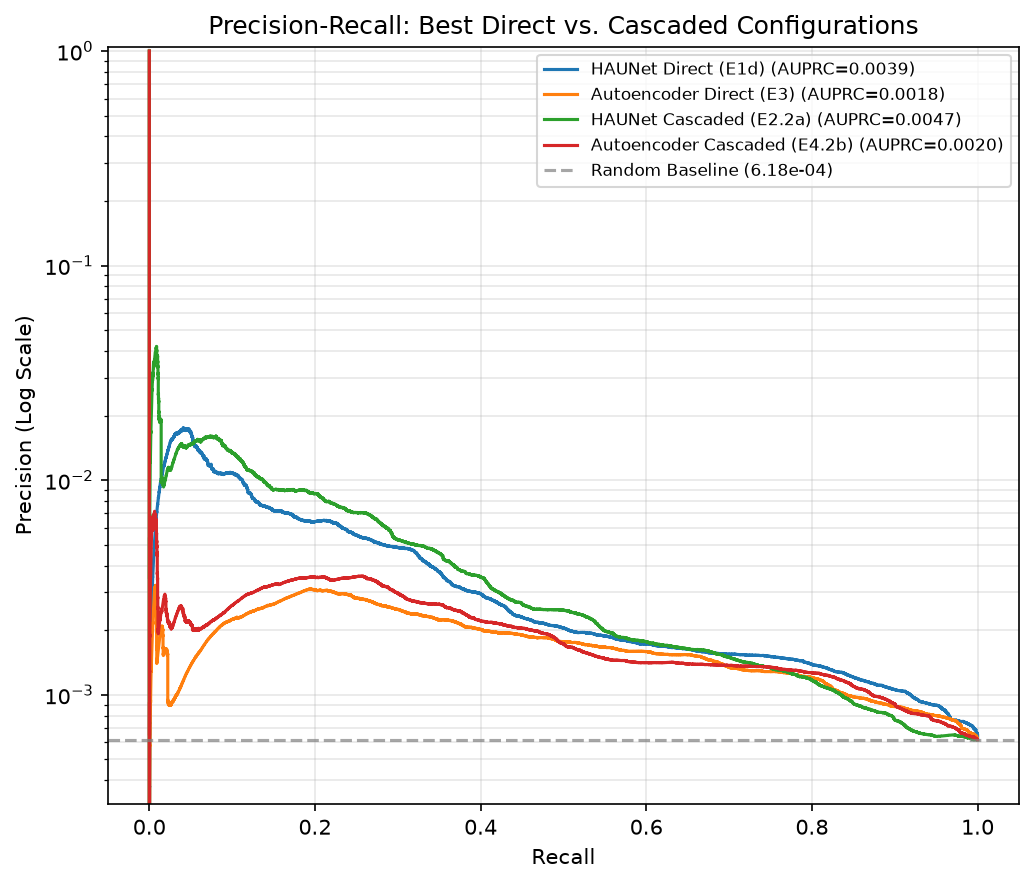
\includegraphics[width=0.85\linewidth]{figures/pr_curve_all_best.png}
    \caption{Precision-Recall curves for best Direct and Cascaded configurations (E1d, E2.2a, E3, E4.2b) against no-skill reference points (Prevalence-Rate = $6.18 \times 10^{-4}$). Curves evaluate raw probability outputs across all decision thresholds.}
    \label{fig:pr_curves}
\end{figure}

% \begin{figure}[htbp]
%     \centering
%     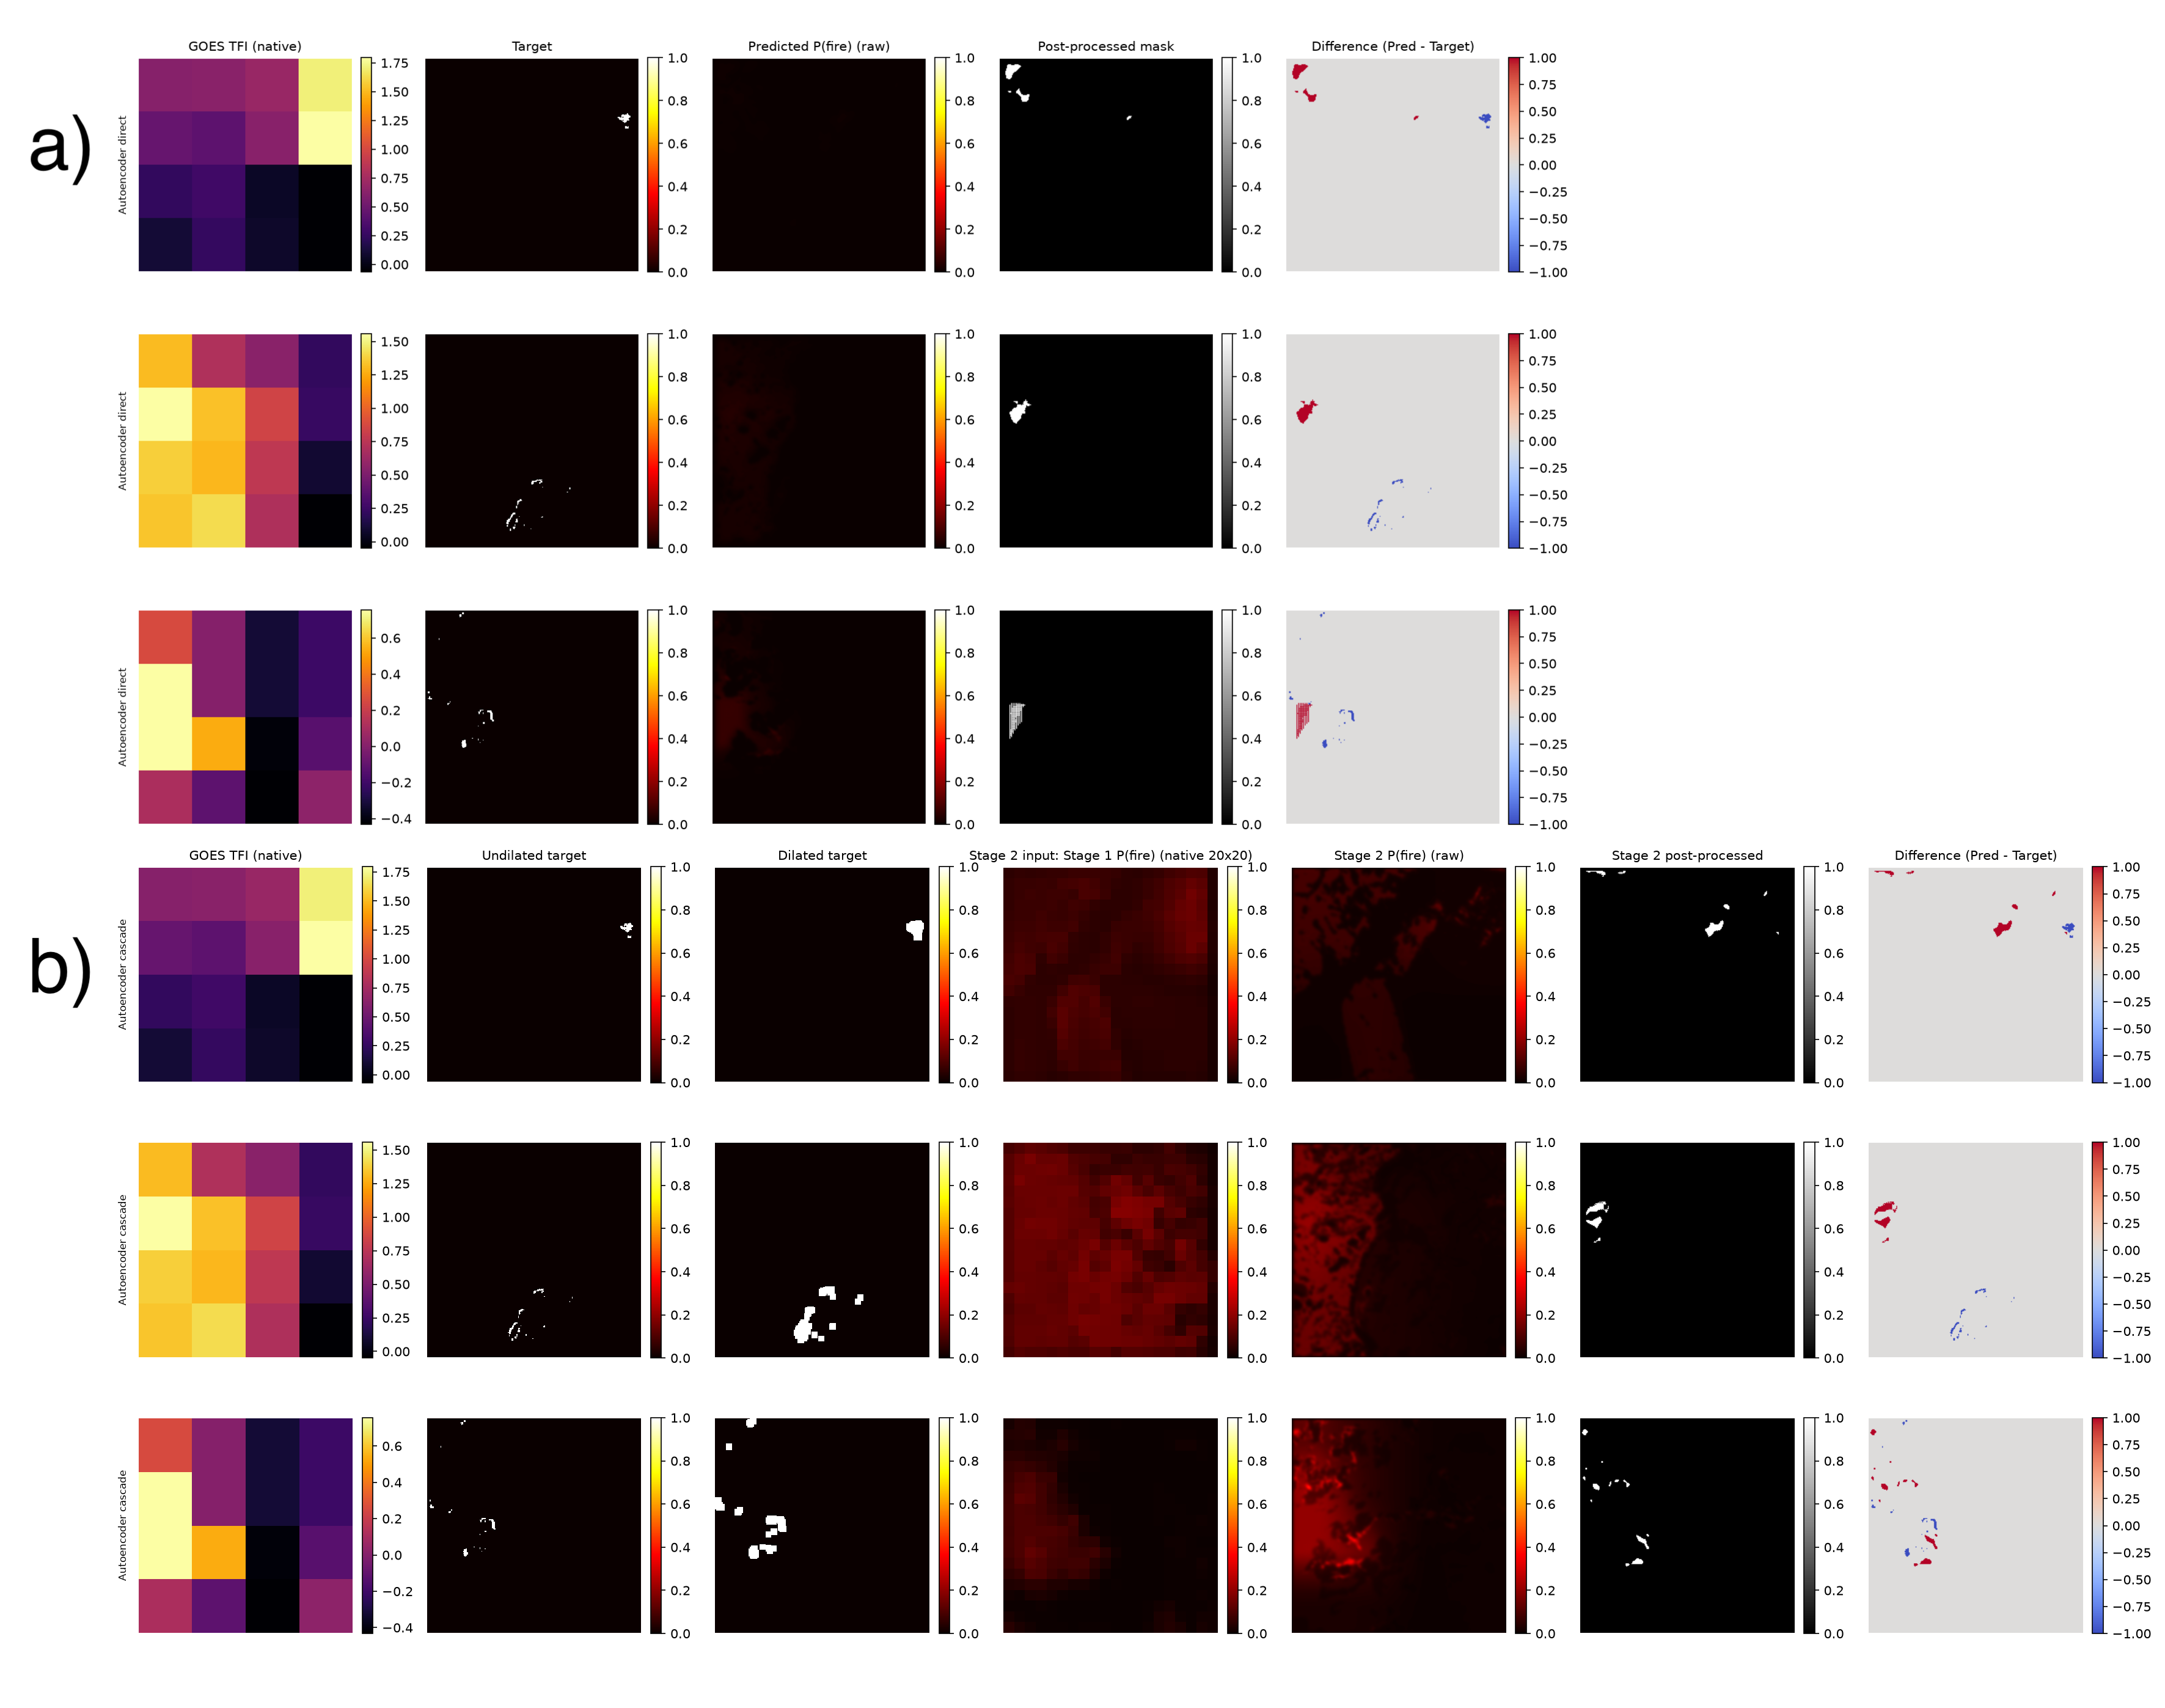
\includegraphics[width=\linewidth]{figures/autoencoder_predictions.png}
%     \caption{Autoencoder direct E3 (a) and cascaded E4.2b (b) prediction examples. From left to right: a) GOES TFI, undilated target, raw predictions, postprocessed predictions, difference. b) input GOES TFI, undilated target, dilated target, Stage 1 prediction, Stage 2 raw prediction, postprocessed prediction, difference.}
%     \label{fig:autoencoder_predictions}
% \end{figure}

% \begin{figure}[htbp]
%     \centering
%     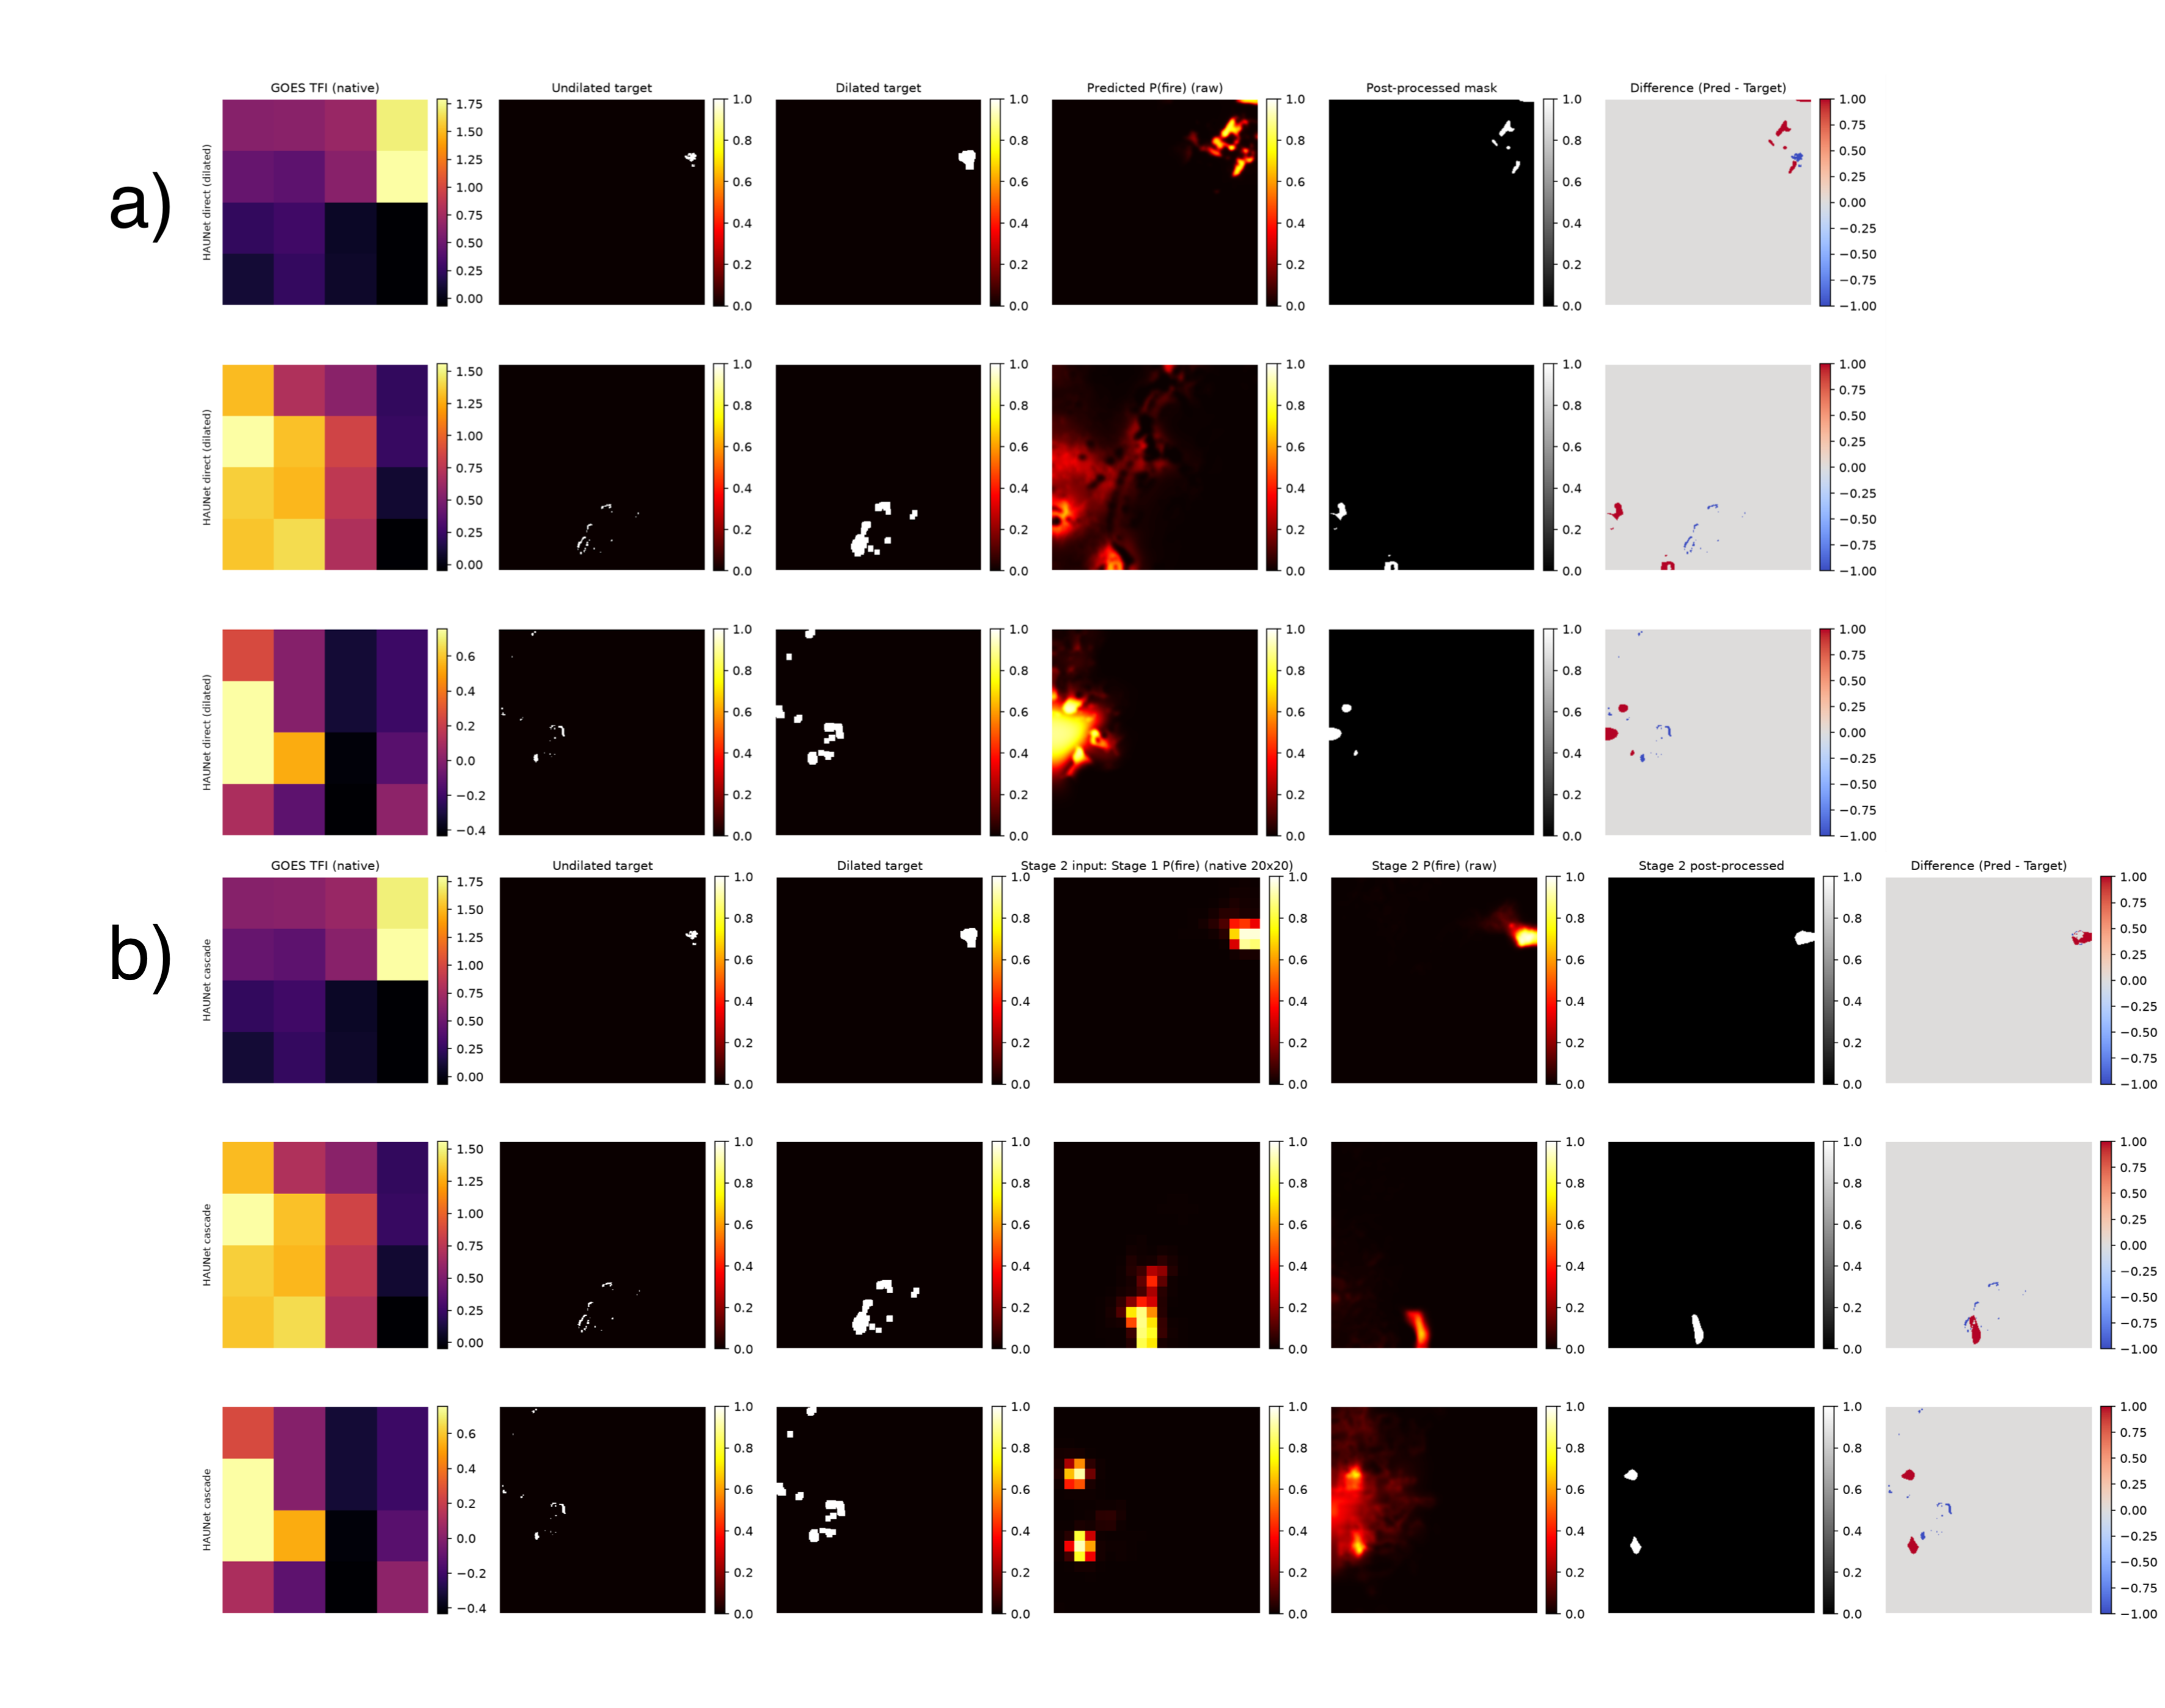
\includegraphics[width=\linewidth]{figures/haunet_predictions.png}
%     \caption{HAUNet direct E1d (a) and cascaded E2.2a (b) prediction examples. From left to right: a) GOES TFI, undilated target, dilated target, raw predictions, postprocessed predictions, difference. b) input GOES TFI, undilated target, dilated target, Stage 1 prediction, Stage 2 raw prediction, postprocessed prediction, difference.}
%     \label{fig:haunet_predictions}
% \end{figure}

\section{Discussions} \label{sec:discussion}

\subsection{Overall Performance}
Across configurations, absolute performance is generally low (most < $0.02$ AUPRC and IOU). But all exceed the no-skill reference points, meaning the models are learning the fire signal rather than predicting background (relative to prevalence, best direct configuration (E1d) achieves an AUPRC of $0.0188$, roughly $30\times$ the reference-point, the best cascaded configuration (E2.2a) roughly $23\times$, and the Autoencoders (E3, E4.2b) roughly $20\times$ and $17\times$ times respectively).

Direct comparison with \cite{badhanDeepLearningApproach2024} is not meaningful given differences in target resolution ($2\,\text{km}$ $\to$ $375\,\text{m}$ vs. $2\,\text{km}$ $\to$ $30\,\text{m}$), prediction target (continuous BT vs. binary fire), and evaluation method. However, their IOU values ($0.03$-$0.24$) achieved with a single smaller resolution jump, less severe class imbalance (20\% fire-coverage threshold, and smaller image $128 \times 128$), and more target dataset (their $5,869$ samples vs. $1,202$ Landsat samples in this study) still results in low overlap. Suggesting the extreme resolution gap and class imbalance in this study make the low absolute performance unsurprising.

95\% CIs were computed for AUPRC via patch-level bootstrap resampling (Table \ref{tab:best_overall}). These are wide relative to the differences between configurations, reflecting the limited test-set size.

\subsection{Over-Prediction, Thresholding, and Practical Implications}
Across most configuration, Recall exceeds Precision (e.g. E1c: Recall $0.5051$ vs. Precision $0.0026$; E1d: Recall $0.3487$ vs. Precision $0.0044$). This indicates the models are over-predicting fire pixels. However, in insurance, over-predicting may be preferable to under-predicting, as false negatives could have more severe consequences than false positives. This pattern is also consistent with \cite{mccarthyDeepLearningApproach2021}, who report high recall with collapsing precision in their GOES-to-VIIRS U-Net, due to hot gases producing false thermal signal around the true fire area. This also raises whether Otsu, which assumes an approximately bimodal score distribution, is optimal for these predictions; it was used for consistency with \cite{badhanDeepLearningApproach2024} and as a parameter-free alternative to fixed threshold. Using a fixed threshold derived from validation PR curve may be worth comparing in future work. The Prevalence-Rate, has no bimodal structure and Otsu collapses to the same all-negative mask as All-Zero, hence identical.

To quantify over-prediction, area inflation ratio was computed (predicted fire area over true fire area). Median inflation ranging from $39\times$ (E2.2a) to $457\times$ (E4.2b) across the four configurations, amplified by extreme rarity of the positive class (Landsat fire pixels comprise only 0.06\% of a patch on average). Note this is a pixel-count ratio than spatial-overlap, it should be read alongside the low IoU values, which already indicate limited spatial localisation.

For Artio's carbon investment risk assessment use case, under-estimating fire is generally more costly than overestimating: the current models are better suited to coarse regional estimates than precise predictions, and any operational use of predicted area would need calibration against this inflation factor. Notably, E2.2a shows lower inflation ($39\times$) than the other configurations, suggesting the cascaded HAUNet may produce more spatially concentrated predictions. Though given the overlapping CIs, this should be treated as observation rather than a confirmed architectural advantage.

\subsection{Cascaded vs. Direct Pipeline}
For HAUNet, Stage 2 (E2.2a: IoU $0.0072$, Precision $0.0074$, AUPRC $0.0142$, Boundary F1 $0.0071$, E2.2b: IOU $0.0089$, Precision $0.0095$, Boundary F1 $0.0104$) outperforms best direct configuration (E1d: IoU $0.0044$, Precision $0.0044$, AUPRC $0.0188$, Boundary F1 $0.0041$) on all metrics except AUPRC and Recall. This suggests the intermediate stage may help the model produce spatially better localised predictions (reflected in overlap-based metrics) but not necessarily improve confidence ranking. Stage 1 metrics are much higher than either Stage 2 or direct-pipeline (e.g. E2.1a AUPRC $0.1458$), but this is due to Stage 1 metric being evaluated at VIIRS target and resolution ($20 \times 20$). So metrics are not directly comparable.

Paired bootstrap test on AUPRC (E2.2a vs. E1d, matched by patch, $1,000$ resamples) gives mean difference of $-0.0042$ with 95\% CI $[-0.0192, 0.0086]$, and E2.2a exceeds E1d in only 30.2\% of resamples. While not significant, it is consistent with the direct configuration retaining an AUPRC advantage, even as the cascaded configuration improves overlap-based metrics. Reinforcing that these two metric families capture different aspects of prediction quality.

For the Autoencoder, there is similar pattern. The direct configuration achieves highest AUPRC (E3: $0.0120$), while cascaded Stage 2 achieve only slightly better IoU and Precision (E4.2a: IoU $0.0065$, Precision $0.0080$ vs. E3: IoU $0.0064$, Precision $0.0077$) and higher Recall (E4.2b: $0.4565$ vs. E3: $0.2592$). Errors from Stage 1 prediction propagate into Stage 2 training inputs, introducing noise that lowers confidence quality (AUPRC).

A paired bootstrap test on AUPRC (E4.2b vs. E3, matched by patch) gives a mean difference of $-0.0013$ with 95\% CI $[-0.0082, 0.0052]$, and E4.2b exceeds E3 in only 32.3\% of resamples, indicating a weaker and less consistent AUPRC gap for the Autoencoder than observed for HAUNet, though neither reaches statistical significance at this sample size.

The divergence between AUPRC and the overlap-based metrics (IoU, Precision, Boundary F1) are seen across comparisons. Because AUPRC is computed over continuous predictions and reflects how well the model ranks pixels by confidence across all thresholds. IoU, Precision, and Boundary F1, are computed only after Otsu thresholding. They depend on the binary mask produced only at one particular threshold. A model can improve performance at specific Otsu threshold (e.g. producing a more spatially coherent, better-localised binary region) without improving its overall confidence across all thresholds. This is a possible explanation for why the cascaded stage, and dilated inputs, improve overlap-based metrics for HAUNet while not improving AUPRC.

\subsection{HAUNet vs. Autoencoder Architecture Comparison}
Comparing best Stage 2 configurations, HAUNet achieves higher AUPRC point estimates than the Autoencoder in both pipelines:
\begin{itemize}
    \item \textbf{Cascaded Pipeline:} HAUNet leads autoencoder on AUPRC (E2.2a: $0.0142$ vs. E4.2a / E4.2b: $0.0106$), IoU (E2.2b: $0.0089$ vs. E4.2a: $0.0065$), Precision ($0.0095$ vs. $0.008$) and Boundary F1 ($0.0104$ vs. $0.004$).
    \item \textbf{Direct Pipeline:} HAUNet leads Autoencoder on AUPRC (E1d: $0.0188$ vs. E3: $0.0120$), Recall ($0.3490$ vs. $0.2592$). While direct Autoencoder achieves higher IoU ($0.0064$ vs. $0.0044$) and Precision ($0.0077$ vs. $0.0044$).

\end{itemize}

Paired bootstrap tests on AUPRC are consistent with this pattern: HAUNet exceeds Autoencoder in 84.2\% of resamples in the direct pipeline (E1d vs. E3, mean diff $+0.0069$, 95\% CI $[-0.0057, 0.0222]$) and 87.1\% in the cascaded pipeline (E2.2a vs. E4.2b, mean diff $+0.0036$, 95\% CI $[-0.0028, 0.0110]$). Both intervals cross zero, so neither comparison is significant at 95\% threshold given the limited test-set size, and this should be read as trend rather than confirmed evidence of an architectural advantage. The consistency of the sign and resample proportion across both pipelines makes HAUNet's edge worth investigating further, but a larger test set would be needed.

Autoencoder predictions produce broader, low-confidence regions (see \ref{fig:autoencoder_predictions_direct} and \ref{fig:autoencoder_predictions_cascaded}), likely due to their convolutional nature. After Otsu thresholding, these wider predictions cover larger ground areas, yielding higher point precision/IoU at the cost of spatial localisation. HAUNet produces sharper predictions with higher overall confidence ranking (PR curves in \ref{fig:pr_curves}). Furthermore, HAUNet Stage 1 provides higher-quality inputs to Stage 2 (E2.1a AUPRC $0.1458$ vs. E4.1 AUPRC $0.0944$) meaning less severe error propagation in the cascaded pipeline. Suggesting the results differ by Stage 2 architecture's own suitability for the task, and differences in the quality of Stage 1 predictions. Investigating these effects require cross-architecture ablation (e.g. evaluating an Autoencoder Stage 2 trained on HAUNet's Stage 1 predictions, vice versa), which is left for future work.

\subsection{Effect of Target Dilation}
Dilating the target improves AUPRC and IoU for HAUNet's direct configuration (E1d vs. E1: AUPRC $0.0188$ vs $0.0103$, IoU $0.0044$ vs $0.0021$) but not for the Autoencoder (E3d vs. E3: AUPRC $0.0098$ vs $0.0120$, IoU $0.0057$ vs $0.0064$, both lower with dilation). This may be because HAUNet's attention mechanisms benefit more from dilation's smoothing/tolerance than the Autoencoder, whose convolutional nature already smooths outputs. This is consistent with the higher recall.

Note that Stage 1 dilation ablation (E2.1a vs. E2.1b) uses smaller kernel matched to the coarser VIIRS grid ($k=3$ vs. $k=7$) and shows AUPRC decrease with dilation ($0.1458$ vs. $0.1408$). This is likely explained by the relative size of the dilation kernel: a $3\times3$ kernel on the $20\times20$ VIIRS grid affects approximately 15\% of the grid dimension, compared to a $7\times7$ kernel on the $256\times256$ Landsat grid, which affects only around 2.7\%. At VIIRS resolution, dilation of this relative magnitude may distort the shape of an already coarse, fire signal rather than providing the tolerance it offers at Landsat resolution. This suggests the appropriate dilation kernel size should be chosen relative to target grid resolution, and that the direct-pipeline dilation effect is not directly comparable to Stage 1.

\subsection{Feature Ablations}
Removing DEM (E1b) produces the weakest performance (AUPRC $0.0050$, IoU $0.0020$ vs. E1: $0.0103$, $0.0021$), and removing land cover (E1c) causes AUPRC drop ($0.0054$) alongside the group's highest Recall ($0.5051$) but lowest Boundary F1 ($0.0020$). Together suggesting both covariates contribute to spatial precision.

Removing the covariate pyramid encoder (E1a) unexpectedly improves overlap-based metrics relative to the full model (IoU: $0.0043$ vs. $0.0021$; Precision: $0.0043$ vs. $0.0021$; Boundary F1: $0.0039$ vs. $0.0030$), while AUPRC is only slightly lower ($0.0098$ vs. $0.0103$). One possible explanation is that without full-resolution covariate detail to sharpen its predictions, the model may default to coarser, more spatially diffuse output, similar in effect to the Autoencoder's convolutional smoothing discussed above. Broader predictions can improve overlap metrics, without necessarily improving the model's overall confidence ranking (reflected in the near-unchanged AUPRC). This may suggest the pyramid encoder's contribution is in sharpening prediction confidence and preserving fine spatial detail rather than in overall discriminative ability. This is worth confirming in future work.

\section{Conclusions}
This project investigated DL pipeline for downscaling GOES imagery into Landsat-resolution wildfire predictions, comparing direct and cascaded mapping across HAUNet and Autoencoder baseline, in the context of Artio's carbon-investment risk assessment use case.

Absolute performance remained modest (AUPRC and IoU $<0.02$), reflecting the extreme resolution gap ($2\,\text{km}$ to $30\,\text{m}$), severe class imbalance, and limited training data ($1,202$ Landsat patches). All configurations exceeded all-zero and prevalence-rate (AUPRC up to $30\times$ the random-classifier) confirming genuine signal extraction rather than deployment-ready accuracy.

No pipeline design showed uniform advantage, and architecture comparisons were pipeline-dependent: in the direct pipeline the Autoencoder achieved better fixed-threshold overlap metrics while HAUNet led on AUPRC and Recall, the cascaded pipeline HAUNet led on every metric. Paired bootstrap tests support consistent AUPRC advantage for HAUNet across both pipelines, though this was not statistically significant at this sample size. This divergence, alongside a large area inflation ratio (up to $457\times$ at Otsu threshold), suggests the current models are better suited to coarse regional risk flagging than precise active fire prediction for Artio's use case. Which has operational relevance, since missed fire is costlier than over-prediction.

Future work should prioritise a cross-architecture ablation isolating Stage 2 performance from Stage 1 input quality, and integration of temporal or climate covariates to move toward operational active fire and intensity prediction.

% ==========================================
%                APPENDIX
% ==========================================
\appendix
\section{Appendix} \label{appendix}

\subsection{Focal Dice Loss Formulation}\label{app:losses}
Focal Loss (\cite{linFocalLossDense2018}) applies $(1 - p_t)^\gamma$ to focus training on sparse positives:
\begin{equation}\label{eq:focal_loss}
    \mathcal{L}_{\text{focal}} = -\alpha_t (1 - p_t)^\gamma \log(p_t)
\end{equation}
where $\alpha_t$ is the balancing factor, $p_t$ is the predicted probability for the ground-truth class, and $p_{i,j} = P(y_{i,j}=1)$ is the estimated probability for the positive class. For a ground-truth label $y_{i,j} \in \{0, 1\}$:
\begin{equation}
    p_t = \begin{cases} 
    p_{i,j} & \text{if } y_{i,j} = 1 \\ 
    1 - p_{i,j} & \text{if } y_{i,j} = 0 
    \end{cases}, \quad 
    \alpha_t = \begin{cases} 
    \alpha & \text{if } y_{i,j} = 1 \\ 
    1 - \alpha & \text{if } y_{i,j} = 0 
    \end{cases}
\end{equation}
$\alpha \in [0, 1]$ balances positive and negative pixel contributions, and $\gamma \ge 0$ controls the rate at which pixels are down-weighted.

Dice Loss (\cite{milletariVNetFullyConvolutional2016}) tries to maximise the spatial overlap:
\begin{equation}\label{eq:dice_loss}
    \mathcal{L}_{\text{dice}} = 1 - \frac{2 \sum_{i,j} p_{i,j} y_{i,j} + \epsilon}{\sum_{i,j} p_{i,j} + \sum_{i,j} y_{i,j} + \epsilon}
\end{equation}
where $\epsilon$ is a smoothing term preventing division by zero.

\subsection{Input GOES and Covariate channels}\label{app:input_plots}
Visual example of the input GOES and covariate channels (inputs used for examples shown in \ref{app:prediction_plots} are shown in Figure \ref{fig:input_reference}.

\begin{figure}[htbp]
    \centering
    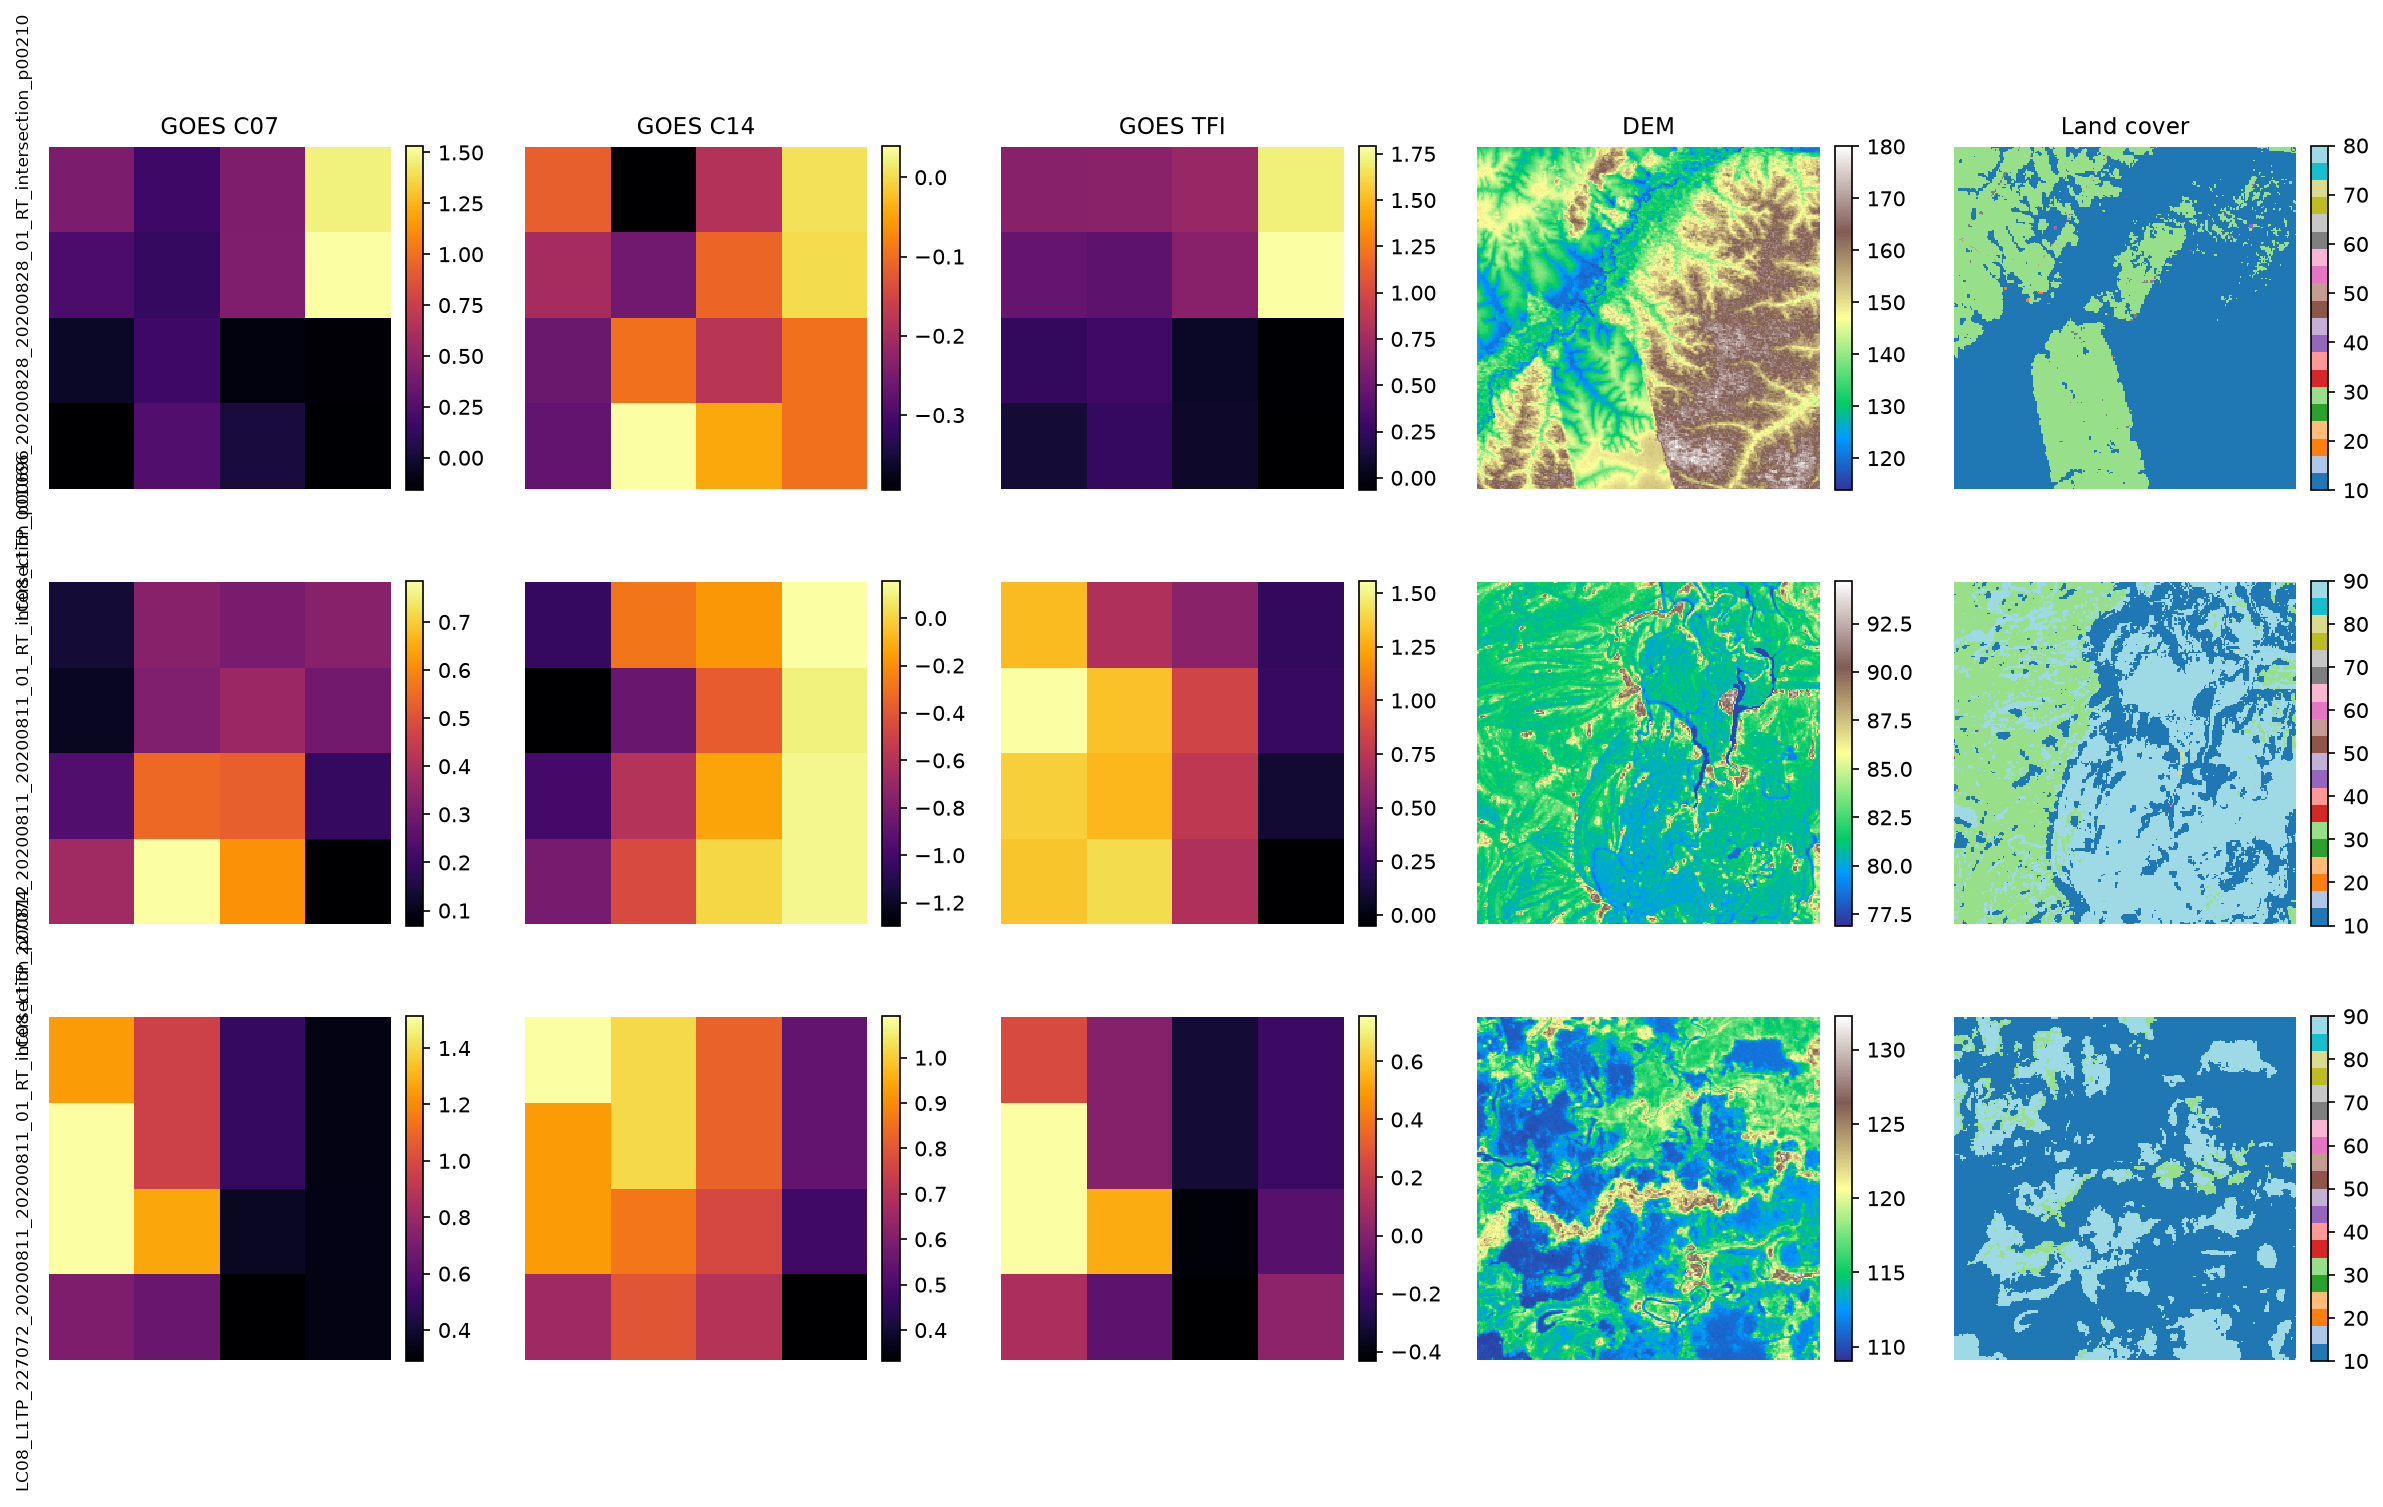
\includegraphics[width=\linewidth]{figures/input_reference.png}
    \caption{GOES and covariates inputs for same samples as figures in \ref{app:prediction_plots}. Left to right: GOES C07, C14, TFI, DEM, Landcover.}
    \label{fig:input_reference}
\end{figure}

\subsection{Prediction Plots}\label{app:prediction_plots}
Figures \ref{fig:autoencoder_predictions_direct} - \ref{fig:haunet_predictions_cascaded} show example predictions for best direct and cascaded HAUNet and Autoencoder models.

\begin{figure}[htbp]
    \centering
    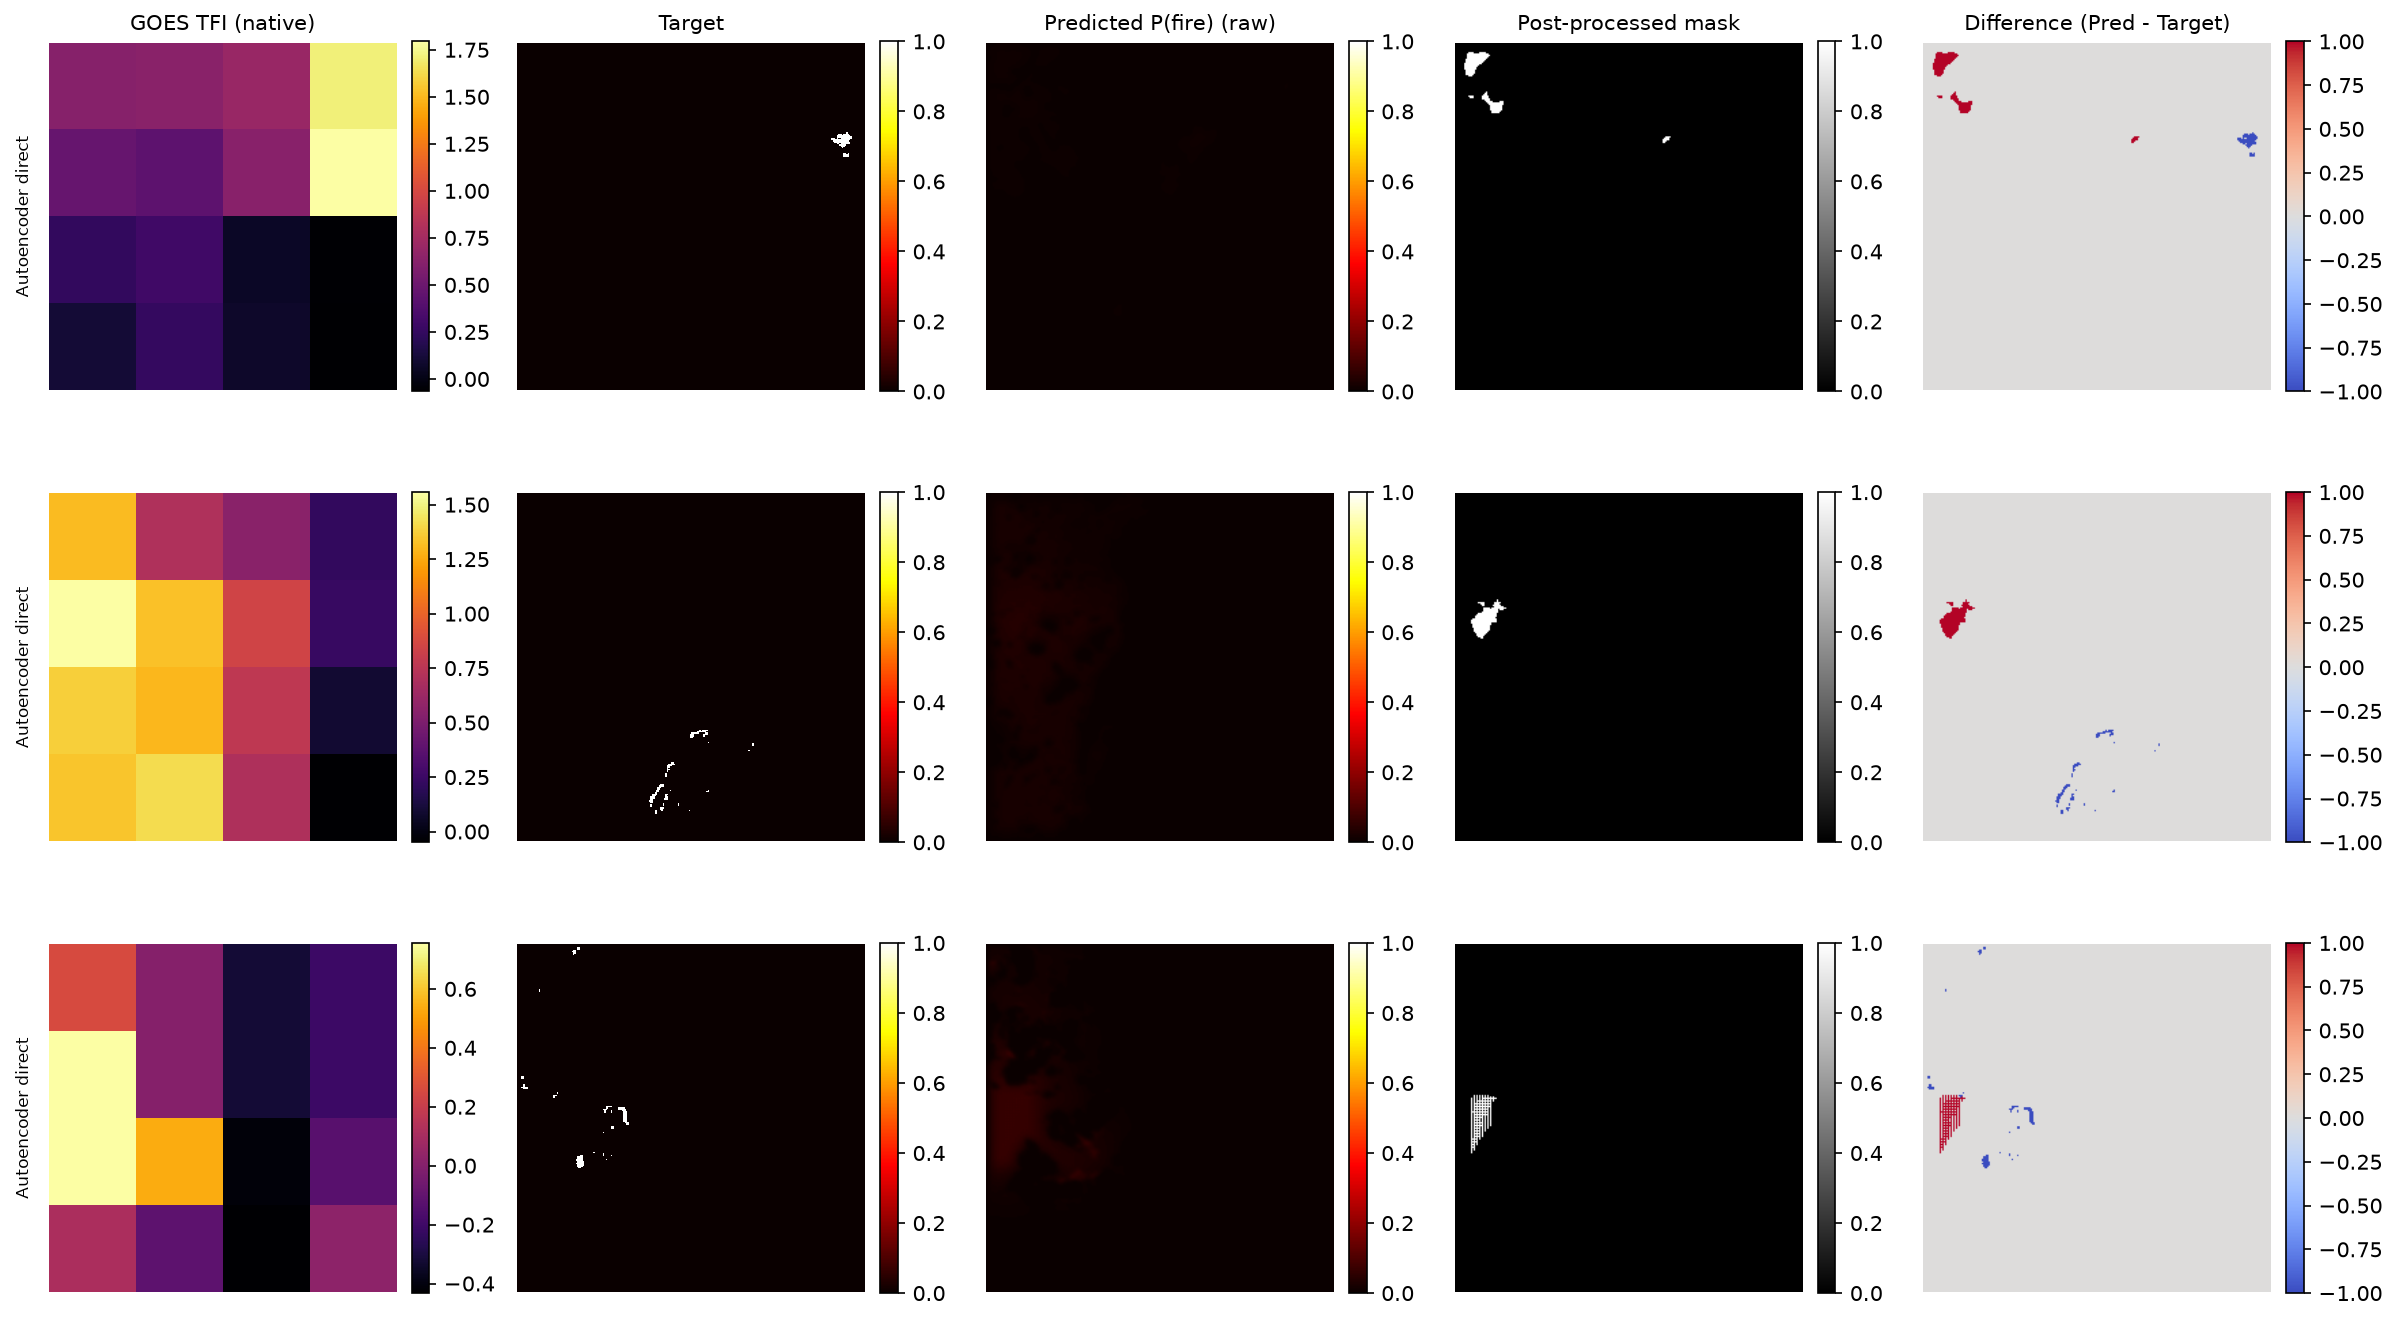
\includegraphics[width=\linewidth]{figures/autoencoder_direct.png}
    \caption{Autoencoder direct (E3) prediction examples. From left to right: GOES TFI, undilated target, dilated target, raw predictions, postprocessed predictions, difference.}
    \label{fig:autoencoder_predictions_direct}
\end{figure}

\begin{figure}[htbp]
    \centering
    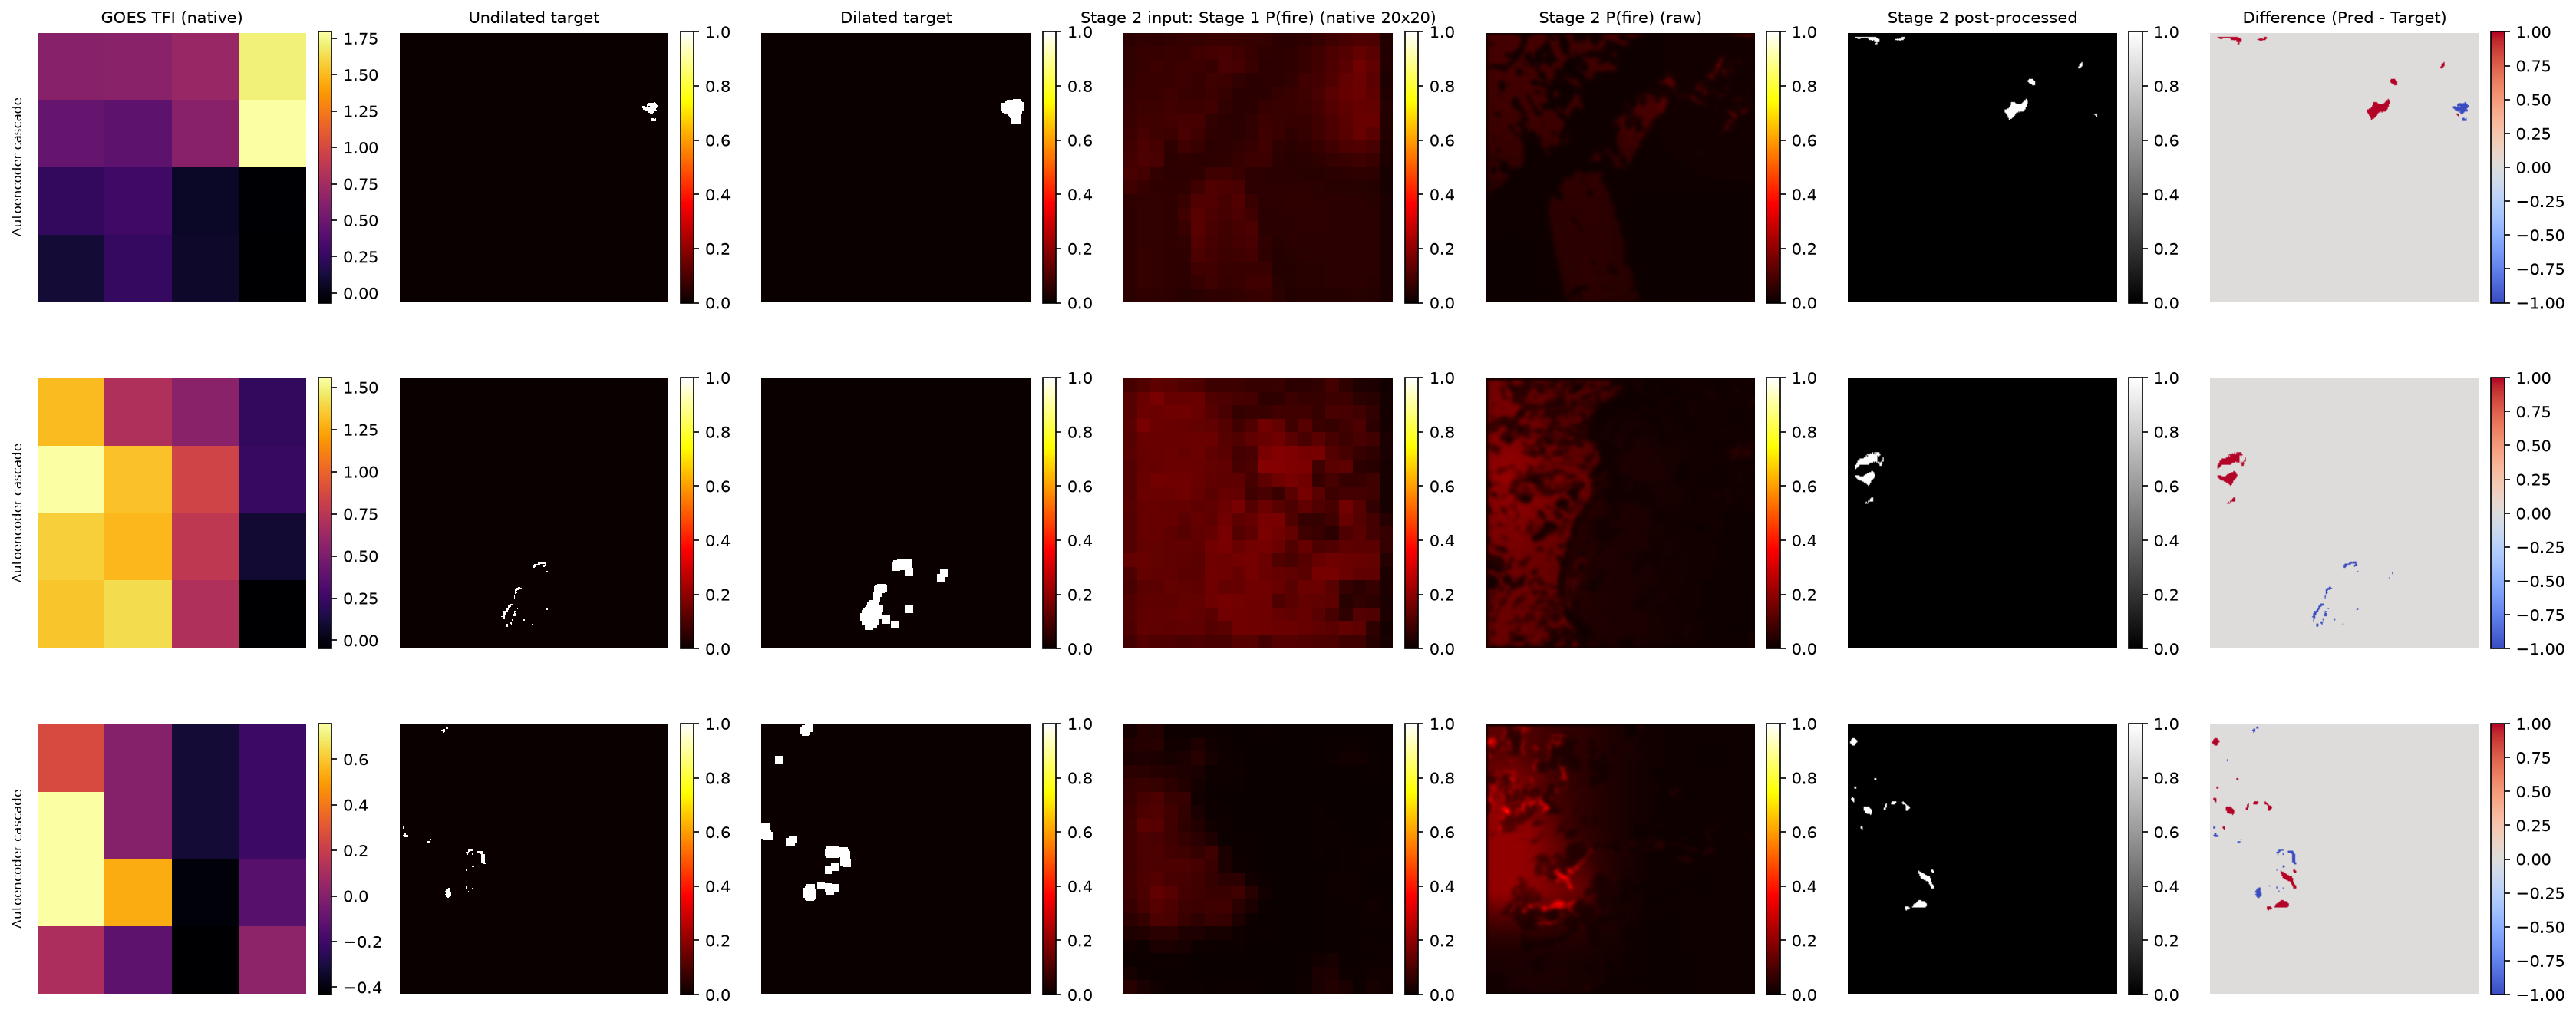
\includegraphics[width=\linewidth]{figures/autoencoder_cascade_dilated.png}
    \caption{Autoencoder cascaded (E4.2b) prediction examples. From left to right: GOES TFI, undilated target, dilated target, raw Stage 1 predictions, raw Stage 2 predictions, postprocessed predictions, difference.}
    \label{fig:autoencoder_predictions_cascaded}
\end{figure}

\begin{figure}[htbp]
    \centering
    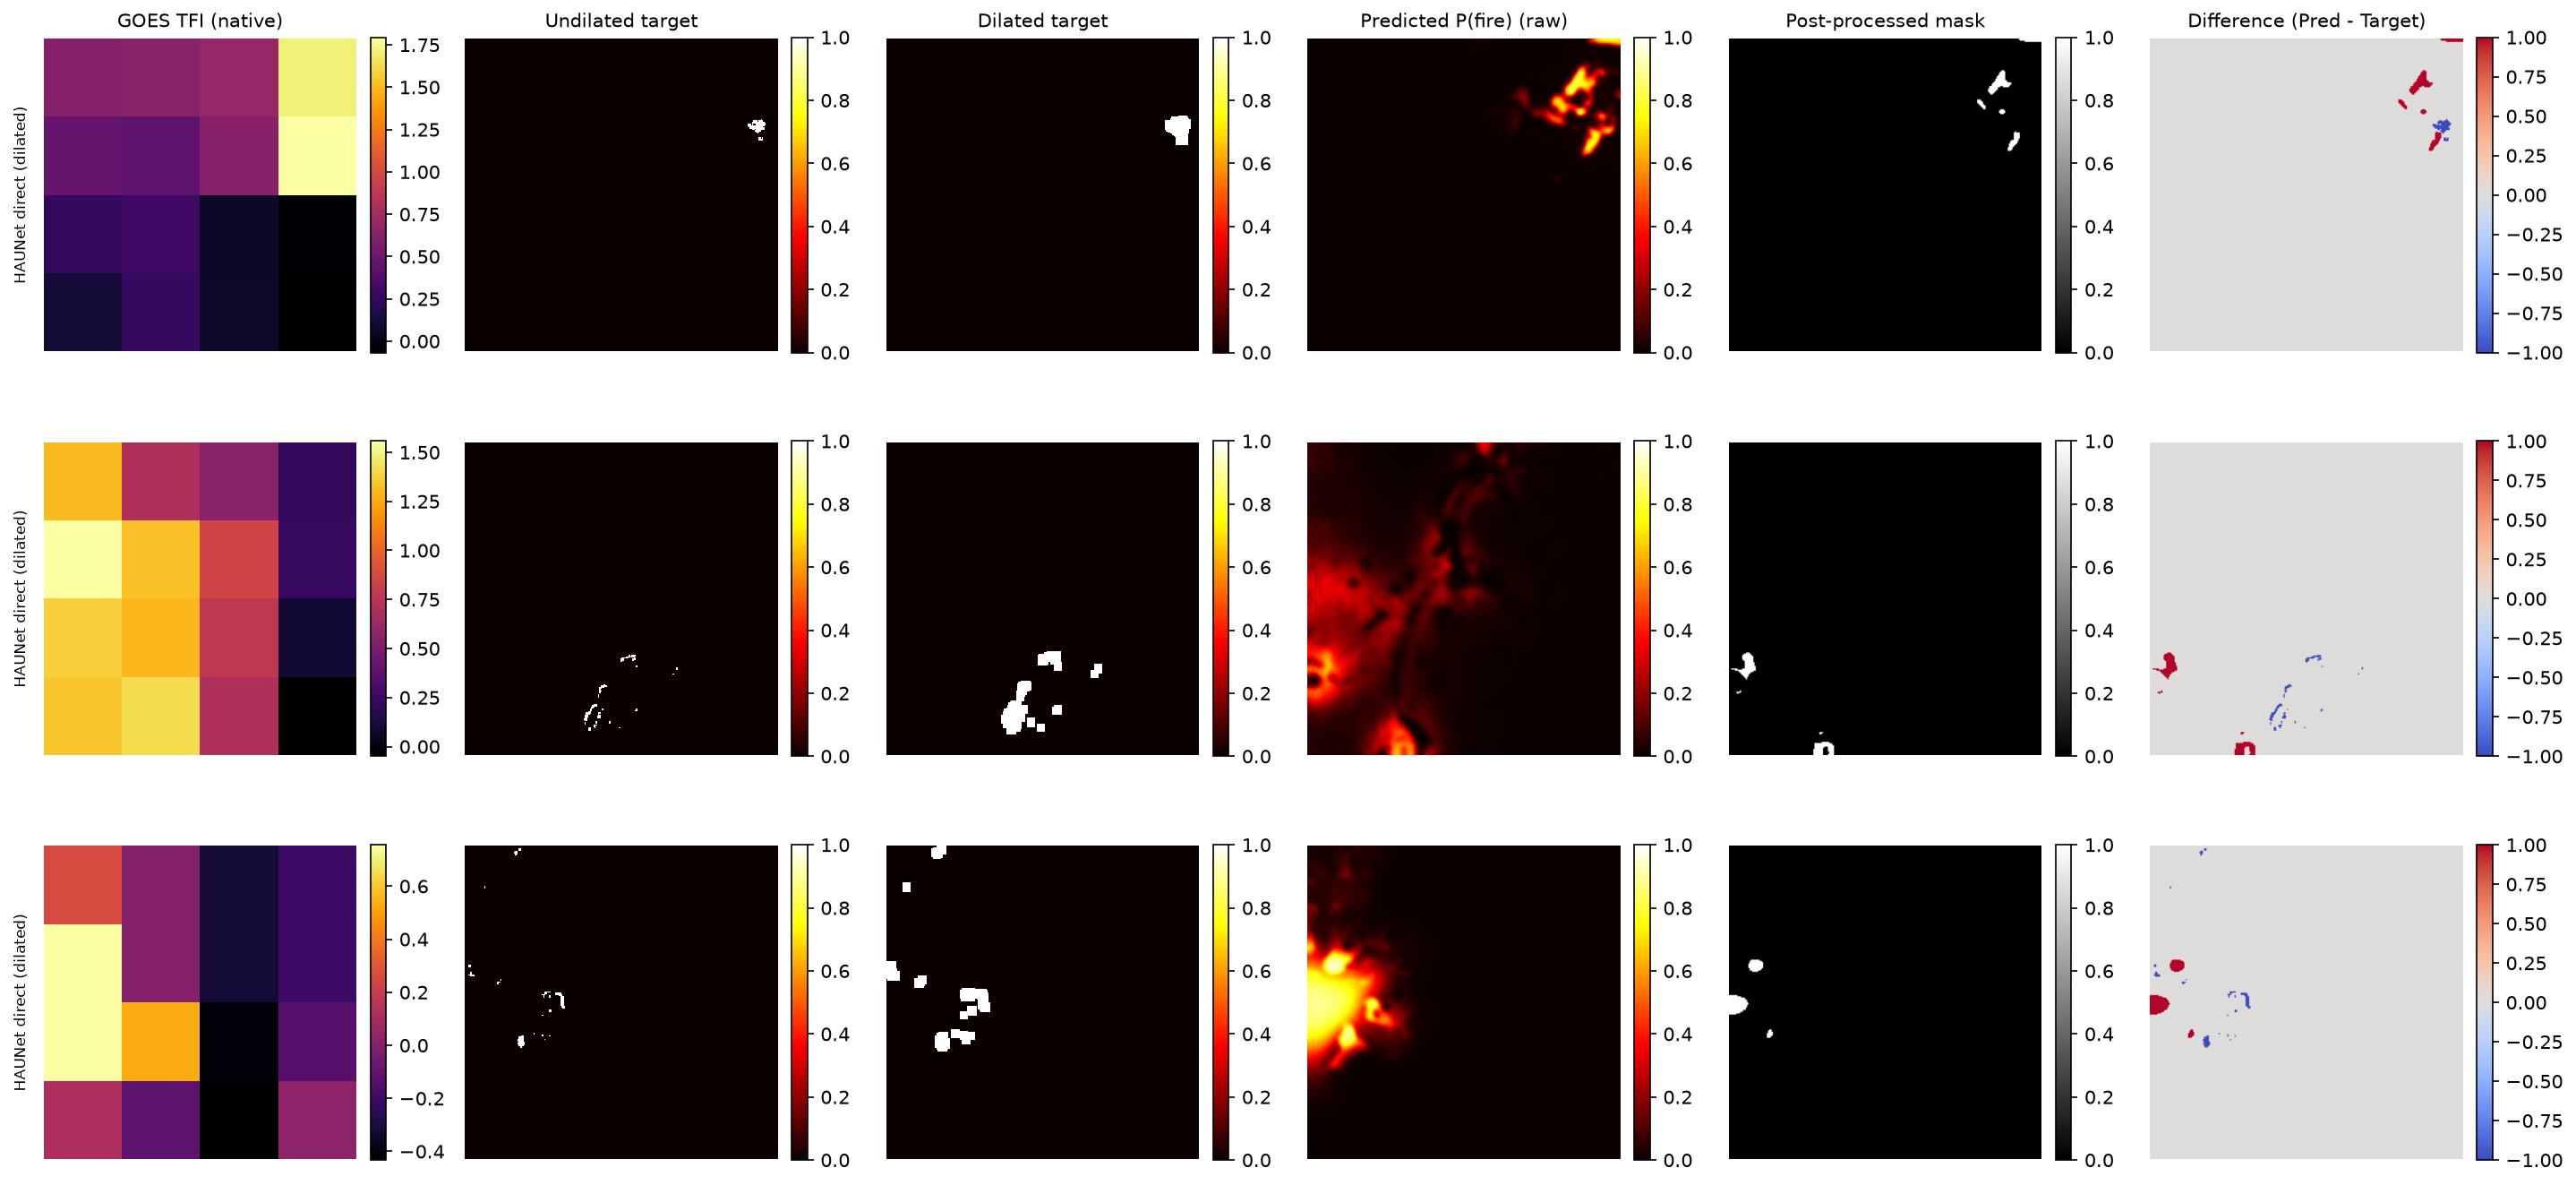
\includegraphics[width=\linewidth]{figures/haunet_direct_dilated.png}
    \caption{HAUNet direct (E1d) prediction examples. From left to right: GOES TFI, undilated target, dilated target, raw predictions, postprocessed predictions, difference.}
    \label{fig:haunet_predictions_direct}
\end{figure}

\begin{figure}[htbp]
    \centering
    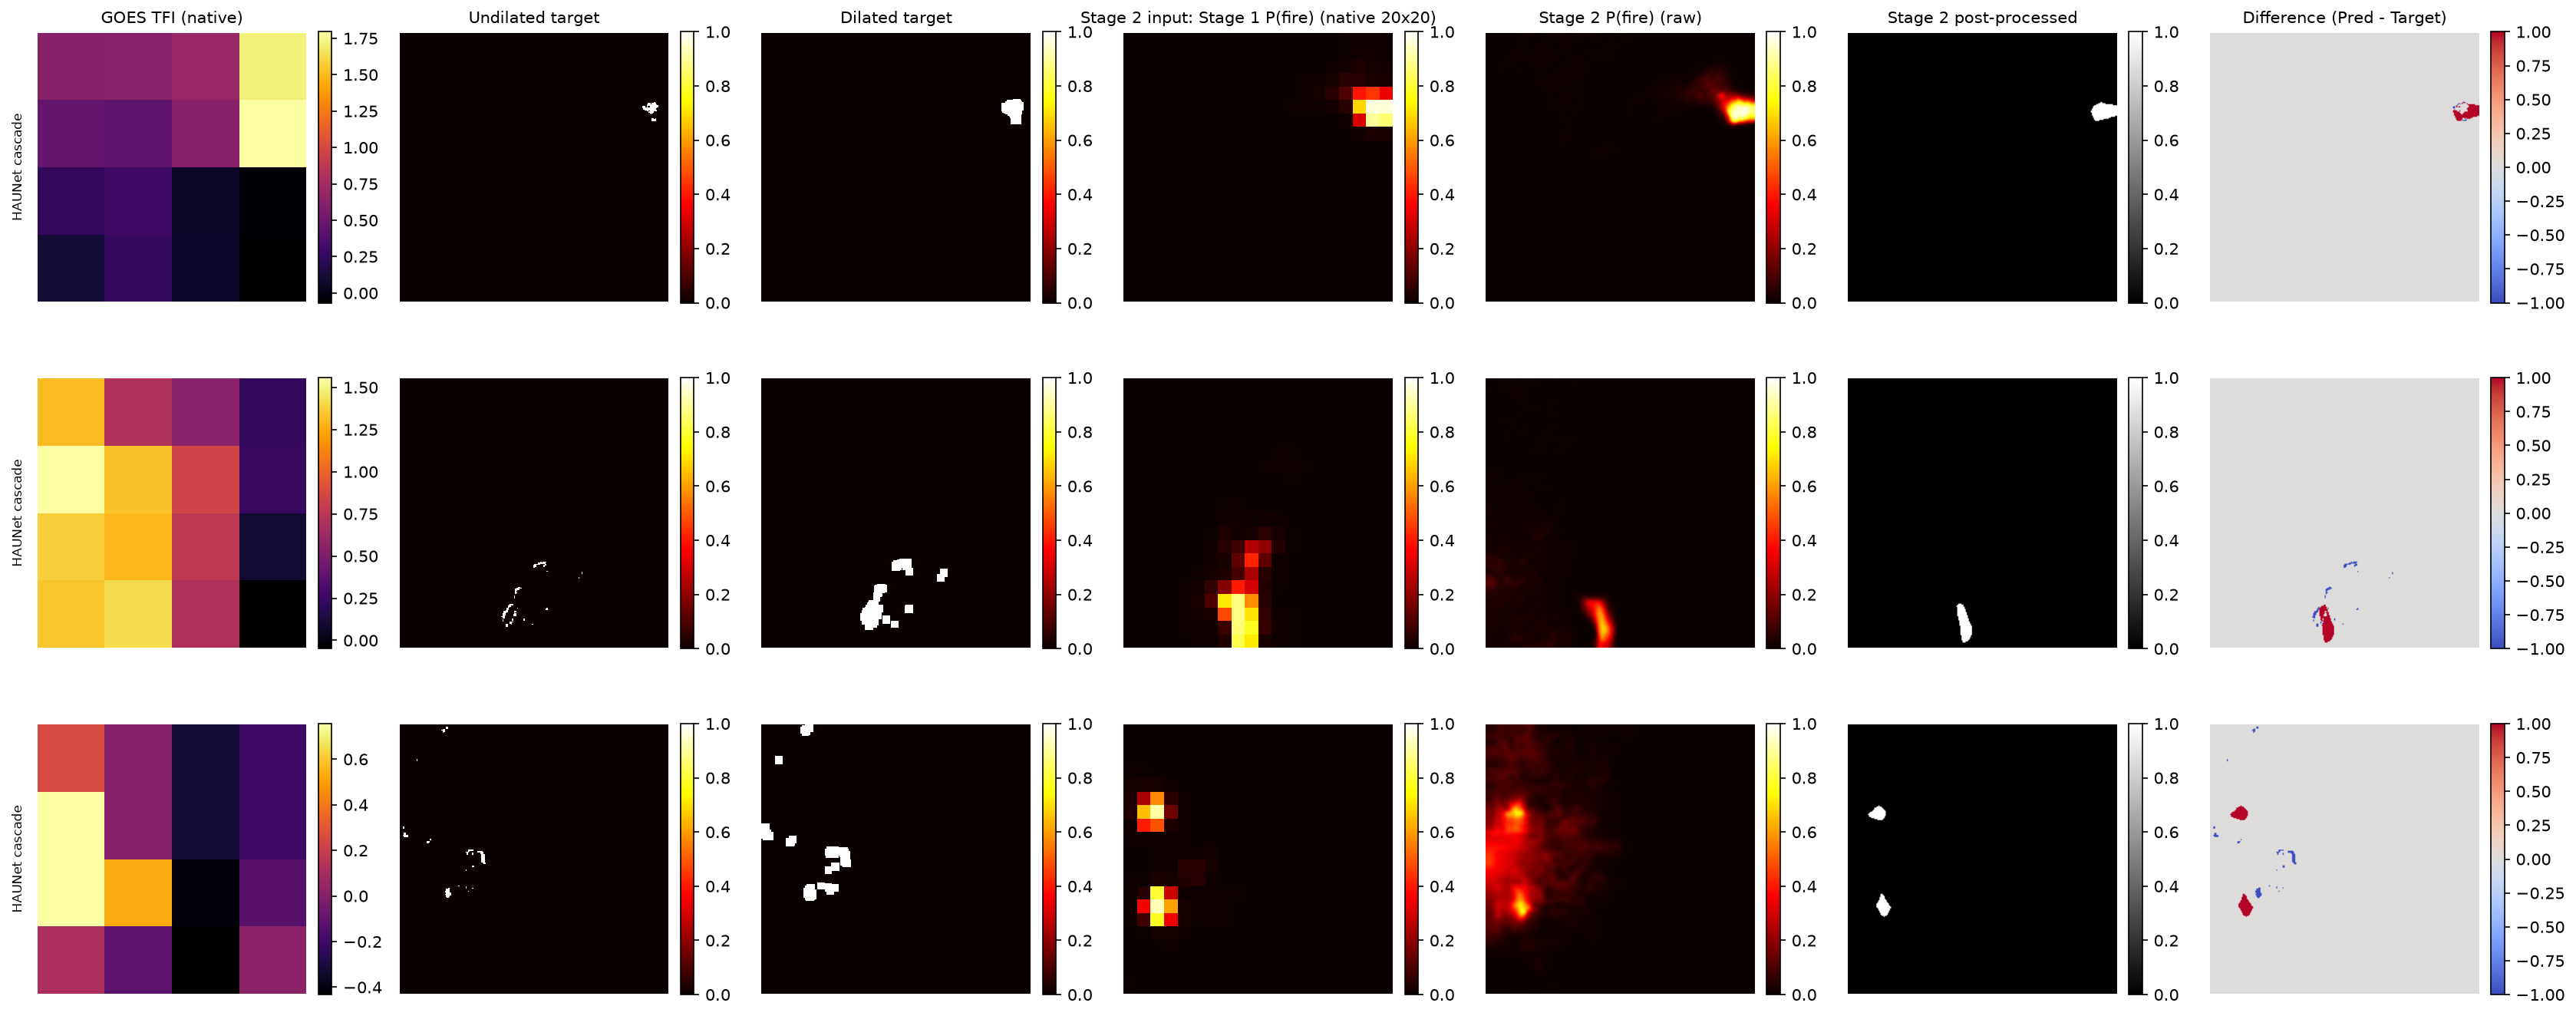
\includegraphics[width=\linewidth]{figures/haunet_cascade_single_dilated.png}
    \caption{HAUNet cascaded (E2.2a) prediction examples. From left to right: GOES TFI, undilated target, dilated target, raw Stage 1 predictions, raw Stage 2 predictions, postprocessed predictions, difference.}
    \label{fig:haunet_predictions_cascaded}
\end{figure}

\printbibliography

\end{document}